%. Author = ktarrant
%. Date = 3/27/23

% Preamble
\documentclass[11pt]{article}

% Packages
\usepackage{amsmath}
\usepackage[T1]{fontenc}%
\usepackage[utf8]{inputenc}%
\usepackage{lmodern}%
\usepackage{textcomp}%
\usepackage{lastpage}%
\usepackage{longtable}%
\usepackage{graphicx}
\usepackage{wrapfig}
\usepackage{mdframed}
\usepackage[default]{gillius}
\usepackage{xcolor}
\graphicspath{ {./imgs/} }

\mdfdefinestyle{PokemonSpotlight}{%
    linecolor=black,
    outerlinewidth=2pt,
    %roundcorner=20pt,
    innertopmargin=4pt,
    innerbottommargin=4pt,
    innerrightmargin=4pt,
    innerleftmargin=4pt,
        leftmargin = 4pt,
        rightmargin = 4pt
    %backgroundcolor=gray!50!white}
        }

% Document
\begin{document}

\section{How To Go To Sinnoh}\label{sec:how-to-go-to-sinnoh}
Talk with Paul in Lilycove city to start the Sinnoh quest.
Check this guide here for a precise walkthrough:
https://pokemonrevolution.net/forum/topic/160991-how-to-get-to-sinnoh/

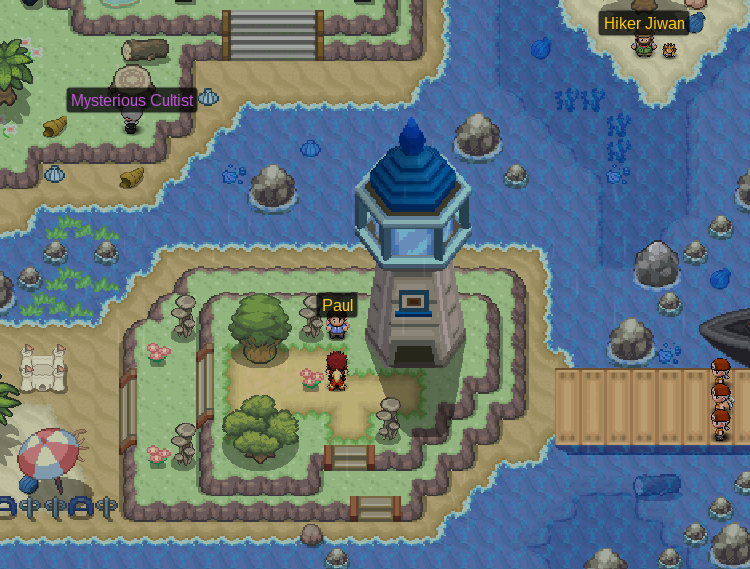
\includegraphics[width=\textwidth]{walkthrough/Sinnoh/paul-lilycove}

\section{Twinleaf Town}\label{sec:twinleaf-town}
Welcome to Sinnoh.
Go downstairs and talk with your grandma.

\section{Route 201}\label{sec:Route_201}
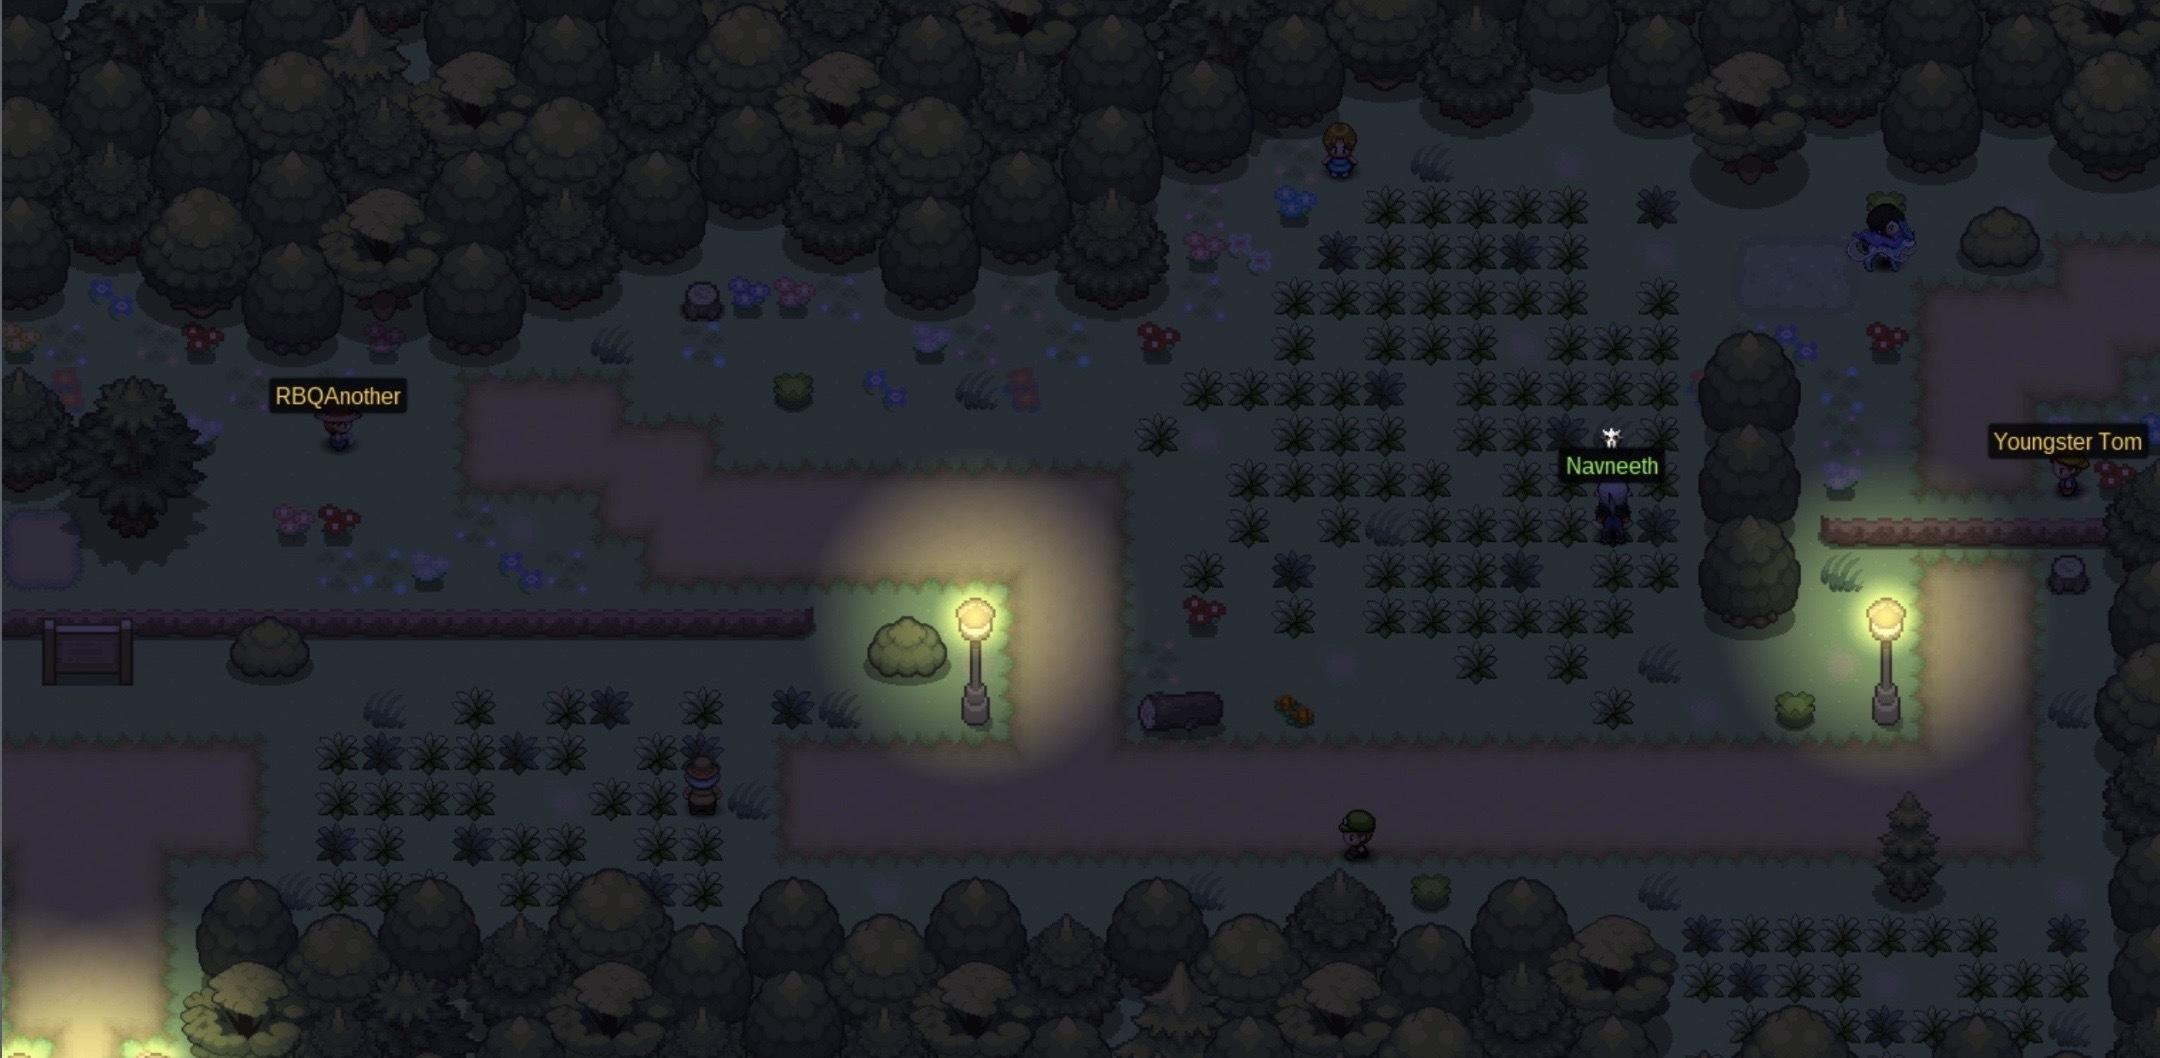
\includegraphics[width=\textwidth]{walkthrough/Sinnoh/Route_201}

Now we can go and visit Barry in his home, go up and talk with him
and then we can meet him in Route 201.

Prof. Rowan is going to stop us from walking in the grass without pokemon
and be ready to choose your starter.

Now go to the right and go to Prof. Rowan lab.

\subsubsection{Wild Pokémon}%
\label{ssubsec:WildPokmon}%
\begin{longtable}{||l l l l l l l l||}%
\hline%
\rowcolor{GroundColor}%
&Pokémon&Level Range&Morn&Day&Night&Held Item&Rarity Tier\\%
\hline%
\endhead%
\hline%
\rowcolor{GroundColor}%

\includegraphics[width=0.02\textwidth]{pokemon/Bidoof}&Bidoof&2{-}4&Morn&Day&Night&&\textcolor{black}{%
Common%
}\\%
\hline%
\rowcolor{GroundColor}%

\includegraphics[width=0.02\textwidth]{pokemon/Doduo}&Doduo&2{-}4&Morn&Day&Night&&\textcolor{black}{%
Common%
}\\%
\hline%
\rowcolor{GroundColor}%

\includegraphics[width=0.02\textwidth]{pokemon/Kricketot}&Kricketot&2{-}4&Morn&Day&Night&&\textcolor{OliveGreen}{%
Uncommon%
}\\%
\hline%
\rowcolor{GroundColor}%

\includegraphics[width=0.02\textwidth]{pokemon/Nidoran F}&Nidoran F&2{-}4&Morn&Day&Night&&\textcolor{black}{%
Common%
}\\%
\hline%
\rowcolor{GroundColor}%

\includegraphics[width=0.02\textwidth]{pokemon/Nidoran M}&Nidoran M&2{-}4&Morn&Day&Night&&\textcolor{black}{%
Common%
}\\%
\hline%
\rowcolor{GroundColor}%

\includegraphics[width=0.02\textwidth]{pokemon/Spritzee}&Spritzee&2{-}4&Morn&Day&Night&&\textcolor{RedOrange}{%
Rare%
}\\%
\hline%
\rowcolor{GroundColor}%

\includegraphics[width=0.02\textwidth]{pokemon/Starly}&Starly&2{-}4&Morn&Day&Night&&\textcolor{black}{%
Common%
}\\%
\hline%
\rowcolor{GroundColor}%

\includegraphics[width=0.02\textwidth]{pokemon/Swirlix}&Swirlix&2{-}4&Morn&Day&Night&&\textcolor{RedOrange}{%
Rare%
}\\%
\hline%
\end{longtable}%
\caption{Wild Pokemon in Route 201}

\begin{mdframed}[style=MyFrame,nobreak=true,frametitle={Pokemon Spotlight: Bidoof}]

The humble Bidoof may not seem like an opposing foe, but some of them are \emph{Moody}.
The Hidden Ability \emph{Moody} raises one of the stats of the Pokémon with this
Ability by two stages (at random), then decreases another stat by one stage (at random).
A Bidoof or Bibarel that stays in battle long enough can reach maxed out stats
and become an unstoppable threat.

\begin{wrapfigure}{l}{0.33\textwidth}
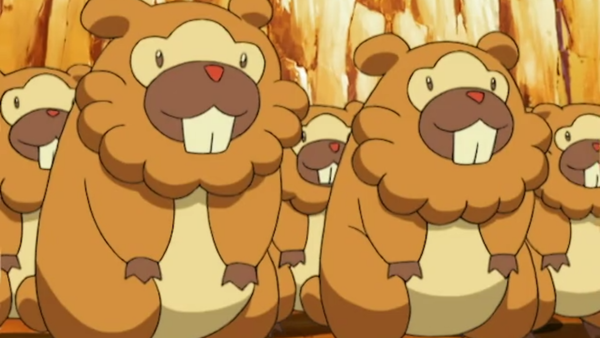
\includegraphics[width=0.33\textwidth]{walkthrough/Sinnoh/spotlight-bidoof}
\label{fig:spotlight-bidoof}
\end{wrapfigure}

The \emph{Moody} ability is perceived as so overpowered that Moody Bibarel has been
banned from most PvP formats.
Although \emph{Moody} will show up in only 5\% of Bidoofs, it may be worth the
grind in the early game to find one with this powerful ability, especially if
you do not pick Piplup as your starter.
The more common ability \emph{Simple} can also be utilized to double the effect of
\emph{Swords Dance} and make Bidoof/Bibarel a threatening foe.
Look for one with an Adamant nature and high IVs in Attack and Speed.

\end{mdframed}

\section{Lake Verity}\label{sec:Lake_Verity}
\subsection{Wild Pokemon}%
\label{subsec:WildPokemon}%
\begin{longtable}{||l l l l l l l l||}%
\hline%
&Pokémon&Level Range&Morn&Day&Night&Held Item&Rarity Tier\\%
\hline%
\endhead%
\hline%

\includegraphics[width=0.05\textwidth]{pokemon/Cherubi}&Cherubi&2{-}5&Morn&Day&Night&&\textcolor{black}{%
Common%
}\\%
\hline%

\includegraphics[width=0.05\textwidth]{pokemon/Psyduck}&Psyduck&2{-}5&Morn&Day&Night&&\textcolor{black}{%
Common%
}\\%
\hline%

\includegraphics[width=0.05\textwidth]{pokemon/Starly}&Starly&2{-}5&Morn&Day&Night&&\textcolor{teal}{%
Uncommon%
}\\%
\hline%

\includegraphics[width=0.05\textwidth]{pokemon/Surskit}&Surskit&2{-}5&Morn&Day&Night&&\textcolor{teal}{%
Uncommon%
}\\%
\hline%

\includegraphics[width=0.05\textwidth]{pokemon/Wynaut}&Wynaut&6{-}9&Morn&Day&Night&&\textcolor{violet}{%
Rare%
}\\%
\hline%
\end{longtable}%
\caption{Lake Verity Wild Pokemon (Land)}%
\begin{longtable}{||l l l l l l l l l||}%
\hline%
&Pokémon&Level Range&Morn&Day&Night&&Held Item&Rarity Tier\\%
\hline%
\endhead%
\hline%

\includegraphics[width=0.05\textwidth]{pokemon/Goldeen}&Goldeen&20{-}30&Morn&Day&Night&&&\textcolor{black}{%
Common%
}\\%
\hline%

\includegraphics[width=0.05\textwidth]{pokemon/Golduck}&Golduck&20{-}30&Morn&Day&Night&&&\textcolor{black}{%
Common%
}\\%
\hline%

\includegraphics[width=0.05\textwidth]{pokemon/Gyarados}&Gyarados&20{-}30&Morn&Day&Night&&&\textcolor{teal}{%
Uncommon%
}\\%
\hline%

\includegraphics[width=0.05\textwidth]{pokemon/Magikarp}&Magikarp&20{-}30&Morn&Day&Night&&&\textcolor{black}{%
Common%
}\\%
\hline%

\includegraphics[width=0.05\textwidth]{pokemon/Psyduck}&Psyduck&20{-}30&Morn&Day&Night&&&\textcolor{black}{%
Common%
}\\%
\hline%

\includegraphics[width=0.05\textwidth]{pokemon/Seaking}&Seaking&20{-}30&Morn&Day&Night&&&\textcolor{teal}{%
Uncommon%
}\\%
\hline%
\end{longtable}%
\caption{Lake Verity Wild Pokemon (Water)}

\section{Sandgem Town}\label{sec:sandgem-town}
Go to the Lab and we will find Barry. He will tell us that he is going to be at Jubilife School.
Enter the Lab and talk with Prof Rowan, But we already have everything from Prof Oak.

\subsection{Back to Grandma}\label{subsec:back-to-grandma}
After talking with Prof. Rowan we cant go to Route 202.
First we need to talk with our Grandma.
Go back to your house and talk with Grandma.
She will tell us that Barry's mom is worried, We need to visit her too.
Talk with his mother and she is going to ask us to tell Barry to go back home, he forgot something.

\section{Route 202}\label{sec:Route_202}

After talking with Grandma and Barry's mom, we can move on to Route 202.

\subsection{Wild Pokemon}%
\label{subsec:WildPokemon}%
\begin{longtable}{||l l l l l l l l||}%
\hline%
&Pokémon&Level Range&Morn&Day&Night&Held Item&Rarity Tier\\%
\hline%
\endhead%
\hline%

\includegraphics[width=0.02\textwidth]{pokemon/Bidoof}&Bidoof&3{-}6&Morn&Day&Night&&\textcolor{black}{%
Common%
}\\%
\hline%

\includegraphics[width=0.02\textwidth]{pokemon/Growlithe}&Growlithe&3{-}6&Morn&Day&Night&&\textcolor{teal}{%
Uncommon%
}\\%
\hline%

\includegraphics[width=0.02\textwidth]{pokemon/Kricketot}&Kricketot&3{-}6&Morn&Day&Night&&\textcolor{teal}{%
Uncommon%
}\\%
\hline%

\includegraphics[width=0.02\textwidth]{pokemon/Sentret}&Sentret&3{-}6&Morn&Day&Night&&\textcolor{black}{%
Common%
}\\%
\hline%

\includegraphics[width=0.02\textwidth]{pokemon/Shinx}&Shinx&3{-}6&Morn&Day&Night&&\textcolor{violet}{%
Rare%
}\\%
\hline%

\includegraphics[width=0.02\textwidth]{pokemon/Starly}&Starly&3{-}6&Morn&Day&Night&&\textcolor{black}{%
Common%
}\\%
\hline%

\includegraphics[width=0.02\textwidth]{pokemon/Zigzagoon}&Zigzagoon&3{-}6&Morn&Day&Night&&\textcolor{black}{%
Common%
}\\%
\hline%
\end{longtable}%
\caption{Route 202 Wild Pokemon (Land)}

\section{Jubilife City}\label{sec:jubilife-city}
Once in Jubilife city we need to find barry in the school.

\subsection{Student Locations}\label{subsec:student-locations}
Unfortunately, Barry is not there and we will have to help the teacher find her students first.

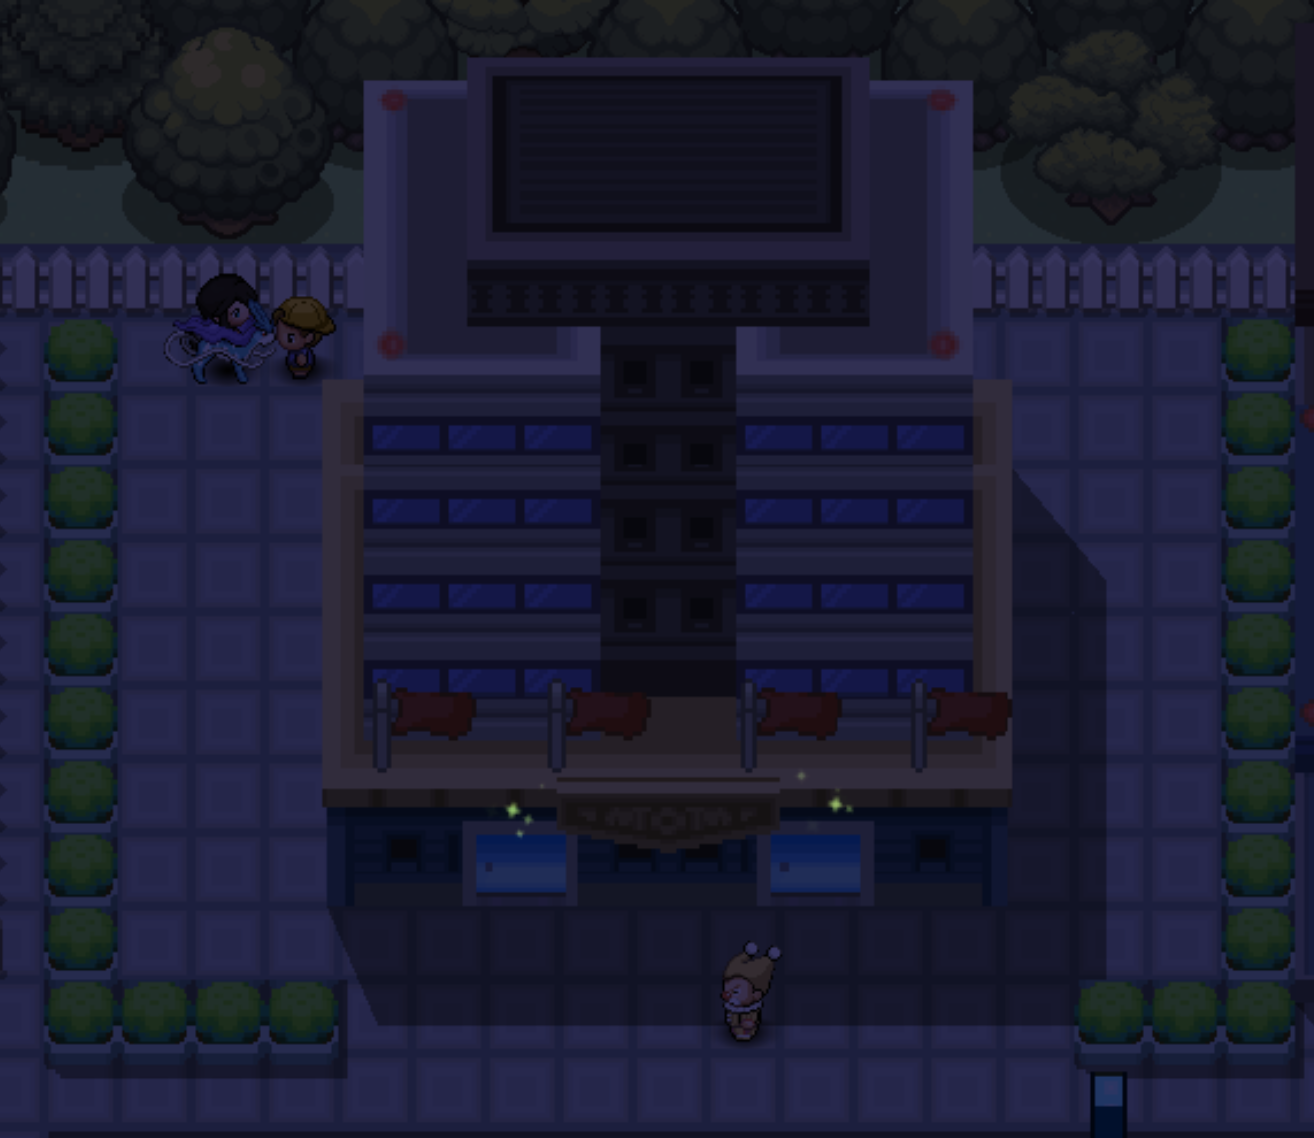
\includegraphics[width=0.5\textwidth]{walkthrough/Sinnoh/Jubilife-student-1}
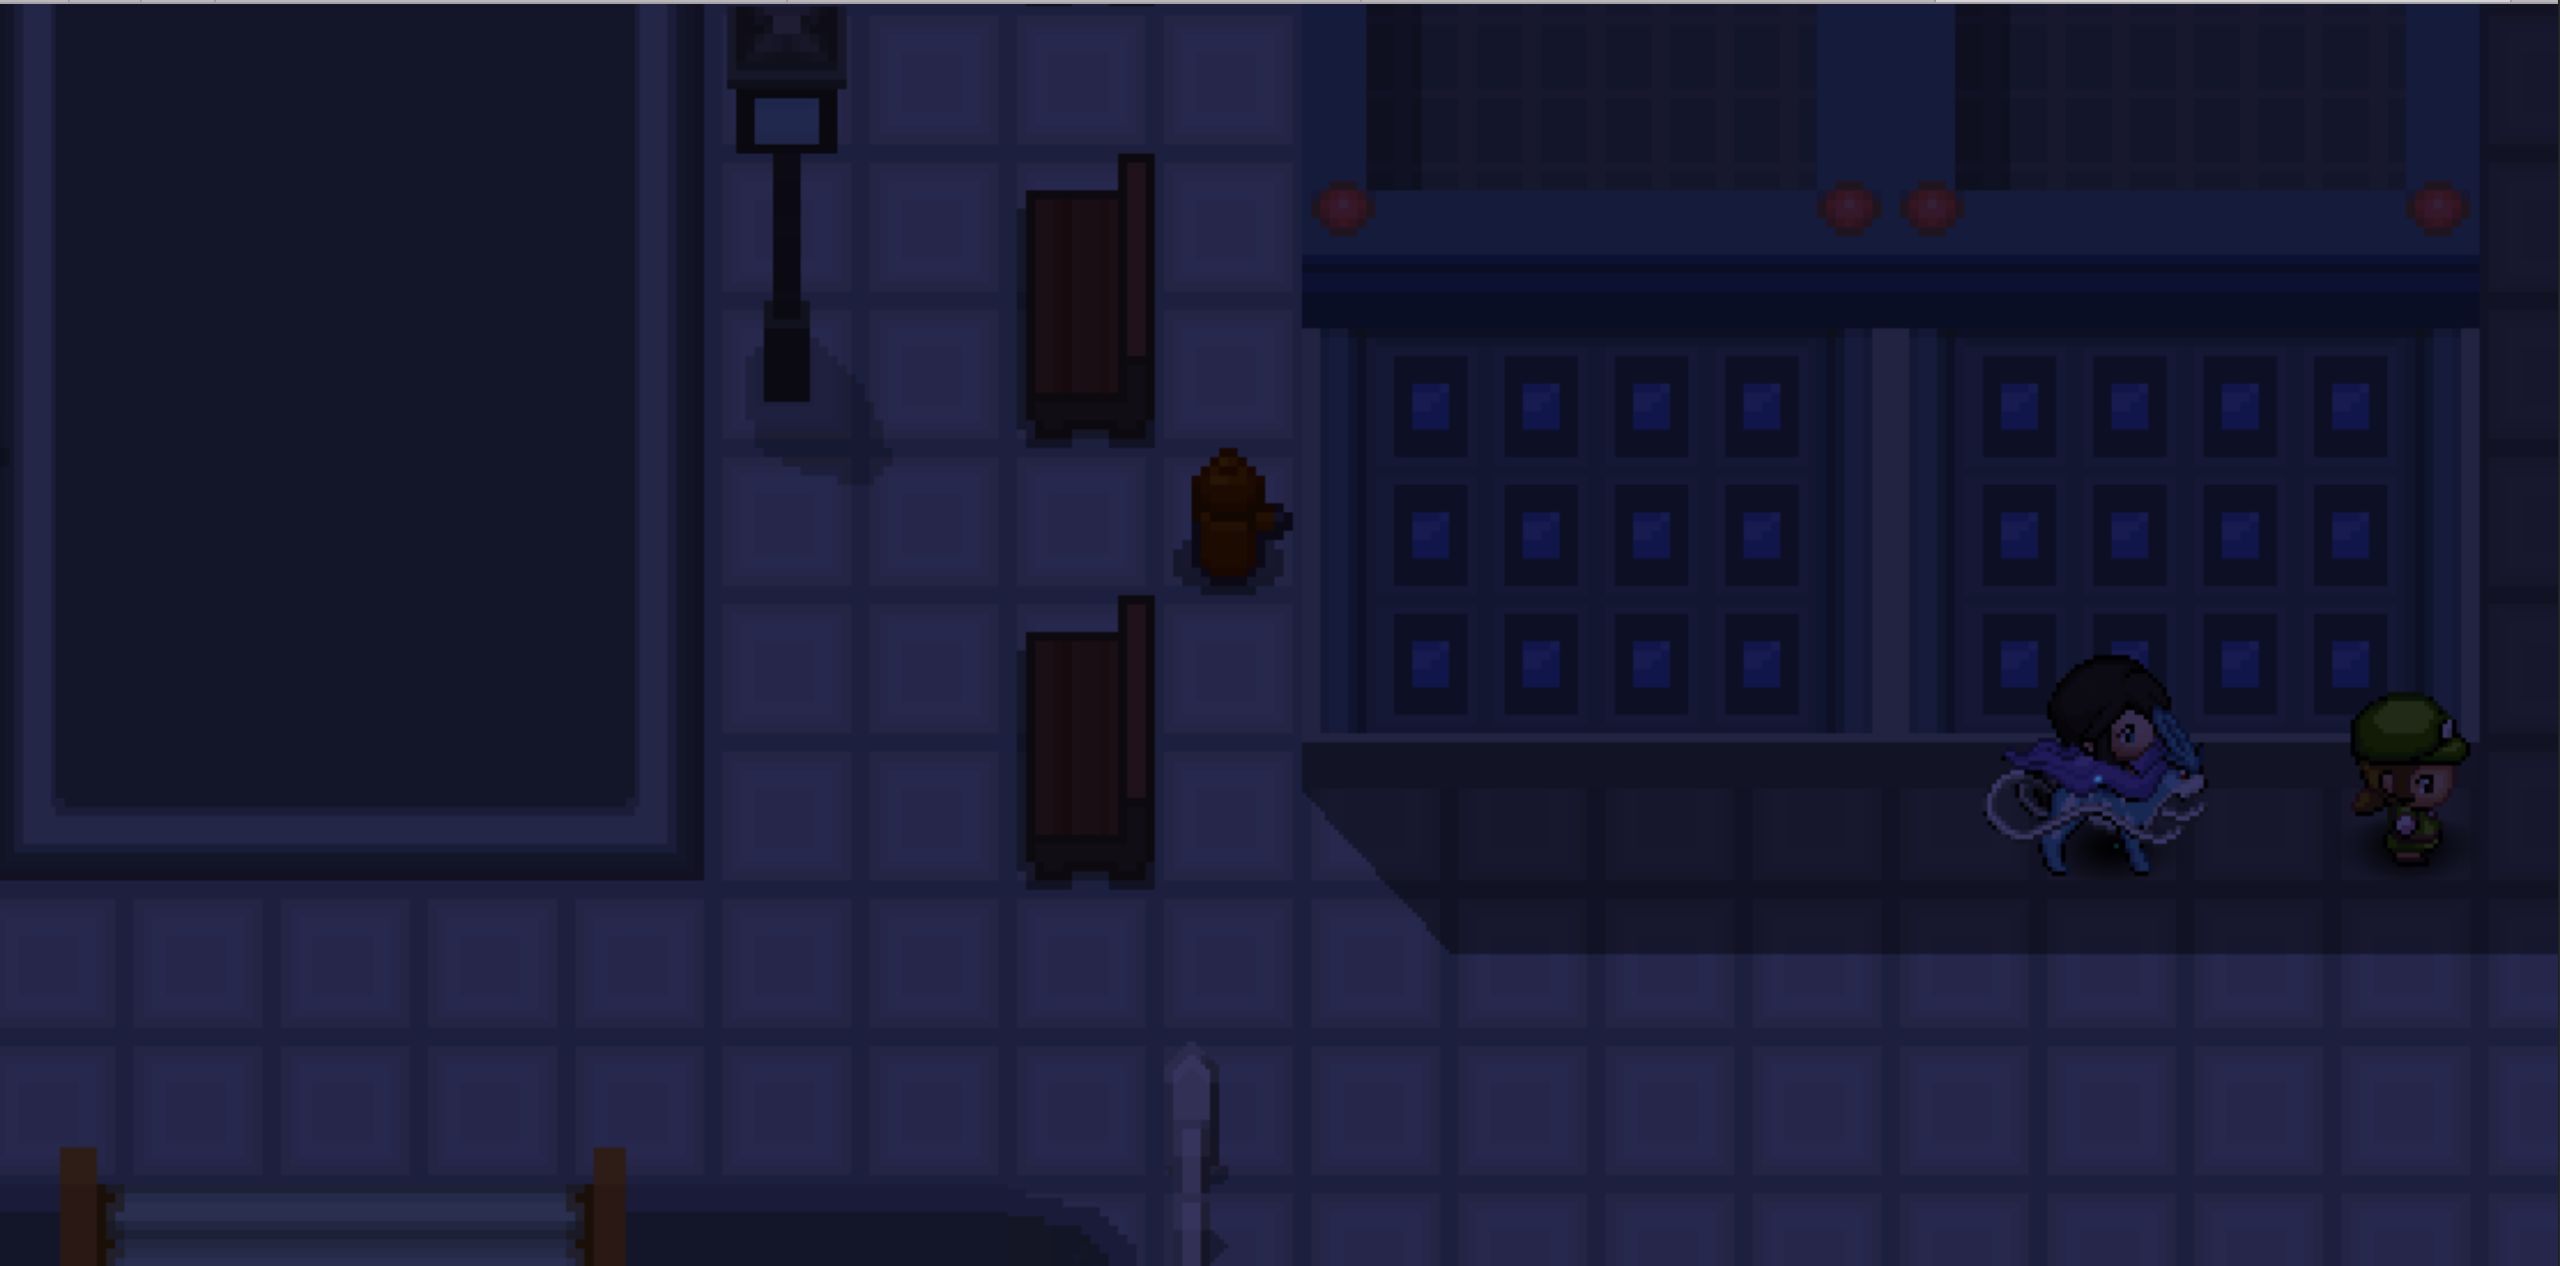
\includegraphics[width=0.5\textwidth]{walkthrough/Sinnoh/Jubilife-student-2}
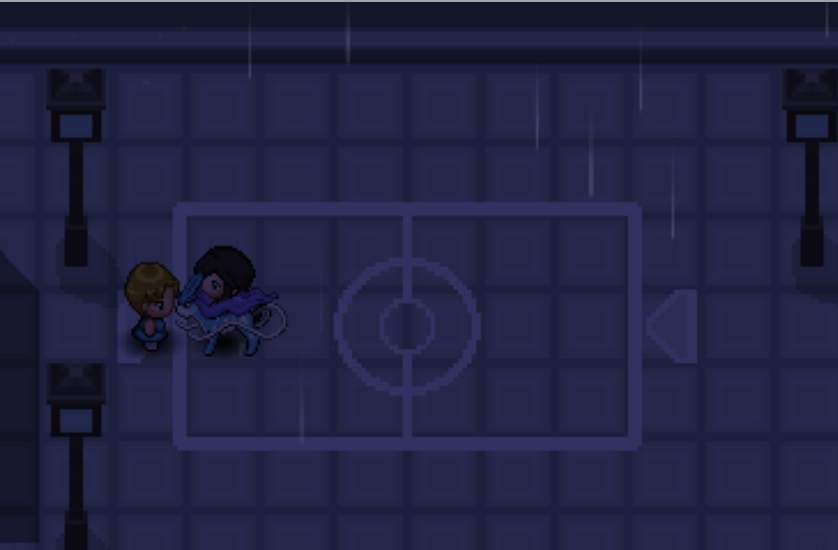
\includegraphics[width=0.5\textwidth]{walkthrough/Sinnoh/Jubilife-student-3}
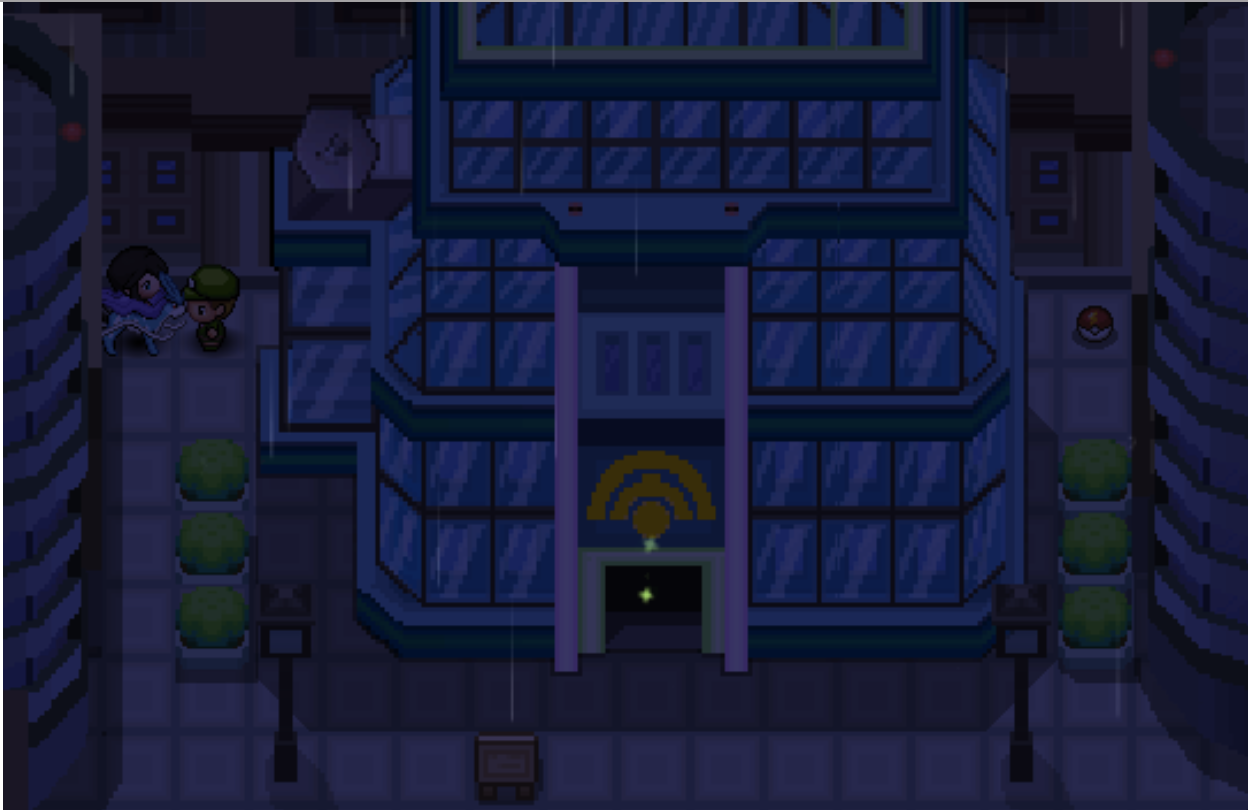
\includegraphics[width=0.5\textwidth]{walkthrough/Sinnoh/Jubilife-student-4}

And then go back to the school and talk with the Teacher.

\section{Route 218}\label{sec:Route_218}

Now we can find Barry at Route 218.
He will go back to his house and then we can go to Route 203.

\subsection{Wild Pokemon}%
\label{subsec:WildPokemon}%
\begin{longtable}{||l l l l l l l l||}%
\hline%
Img&Pokémon&Level Range&Morning&Day&Night&Held Item&Rarity Tier\\%
\hline%
\endhead%
\hline%
&Chatot&28{-}31&Morning&Day&Night&&Rare\\%
\hline%
&Combee&28{-}31&Morning&Day&Night&Honey&Uncommon\\%
\hline%
&Ditto&28{-}31&Morning&&Night&&Uncommon\\%
\hline%
&Shellos&32{-}35&Morning&Day&Night&&Rare\\%
\hline%
&Spoink&28{-}31&Morning&Day&Night&Persim Berry&Uncommon\\%
\hline%
&Starly&25{-}28&Morning&Day&Night&&Common\\%
\hline%
&Timburr&32{-}35&Morning&&Night&&Rare\\%
\hline%
&Vespiquen&28{-}31&Morning&Day&Night&Honey&Uncommon\\%
\hline%
\end{longtable}%
\begin{longtable}{||l l l l l l l l l||}%
\hline%
Img&Pokémon&Level Range&Morning&Day&Night&Rod&Held Item&Rarity Tier\\%
\hline%
\endhead%
\hline%
&Finneon&28{-}31&Morning&Day&Night&&&Uncommon\\%
\hline%
&Gyarados&28{-}31&Morning&Day&Night&&&Uncommon\\%
\hline%
&Lumineon&28{-}31&Morning&Day&Night&&&Uncommon\\%
\hline%
&Magikarp&28{-}31&Morning&Day&Night&&&Common\\%
\hline%
&Pelipper&28{-}31&Morning&Day&Night&&&Uncommon\\%
\hline%
&Shellos&28{-}31&Morning&Day&Night&&&Rare\\%
\hline%
&Tentacool&28{-}31&Morning&Day&Night&&&Common\\%
\hline%
&Tentacruel&28{-}31&Morning&Day&Night&&&Common\\%
\hline%
&Wingull&28{-}31&Morning&Day&Night&&&Common\\%
\hline%
\end{longtable}

\section{Route 203}\label{sec:Route_203}

Be ready to battle with Barry.
Beat him and enter the cave in the right.

\subsection{Wild Pokemon}%
\label{subsec:WildPokemon}%
\begin{longtable}{||l l l l l l l l||}%
\hline%
Img&Pokémon&Level Range&Morning&Day&Night&Held Item&Rarity Tier\\%
\hline%
\endhead%
\hline%
&Abra&2{-}4&Morning&Day&Night&&Uncommon\\%
\hline%
&Aromatisse&2{-}4&Morning&Day&Night&&Rare\\%
\hline%
&Bidoof&2{-}4&Morning&Day&Night&&Common\\%
\hline%
&Kricketot&2{-}4&Morning&Day&Night&&Uncommon\\%
\hline%
&Riolu&5&Morning&&Night&&Rare\\%
\hline%
&Shinx&2{-}4&Morning&Day&Night&&Rare\\%
\hline%
&Starly&2{-}4&Morning&Day&Night&&Common\\%
\hline%
&Zubat&2{-}4&&&Night&&Common\\%
\hline%
\end{longtable}%
\begin{longtable}{||l l l l l l l l l||}%
\hline%
Img&Pokémon&Level Range&Morning&Day&Night&Rod&Held Item&Rarity Tier\\%
\hline%
\endhead%
\hline%
&Goldeen&20{-}35&Morning&Day&Night&&&Common\\%
\hline%
&Golduck&20{-}35&Morning&Day&Night&&&Common\\%
\hline%
&Gyarados&20{-}35&Morning&Day&Night&&&Uncommon\\%
\hline%
&Magikarp&20{-}35&Morning&Day&Night&&&Common\\%
\hline%
&Psyduck&20{-}35&Morning&Day&Night&&&Common\\%
\hline%
&Seaking&20{-}35&Morning&Day&Night&&&Uncommon\\%
\hline%
\end{longtable}

\section{Oreburgh Gate}\label{sec:oreburgh-gate}

Ignore the upper route for now and go to the right.

\subsection{Wild Pokemon}%
\label{subsec:WildPokemon}%
\begin{longtable}{||l l l l l l l l||}%
\hline%
&Pokémon&Level Range&Morn&Day&Night&Held Item&Rarity Tier\\%
\hline%
\endhead%
\hline%

\includegraphics[width=0.02\textwidth]{pokemon/Ducklett}&Ducklett&5{-}9&Morn&Day&Night&&\textcolor{teal}{%
Uncommon%
}\\%
\hline%

\includegraphics[width=0.02\textwidth]{pokemon/Hariyama}&Hariyama&5{-}9&Morn&Day&Night&&\textcolor{teal}{%
Uncommon%
}\\%
\hline%

\includegraphics[width=0.02\textwidth]{pokemon/Hoothoot}&Hoothoot&5{-}9&Morn&Day&Night&&\textcolor{black}{%
Common%
}\\%
\hline%

\includegraphics[width=0.02\textwidth]{pokemon/Makuhita}&Makuhita&5{-}9&Morn&Day&Night&&\textcolor{teal}{%
Uncommon%
}\\%
\hline%

\includegraphics[width=0.02\textwidth]{pokemon/Noctowl}&Noctowl&5{-}9&Morn&Day&Night&&\textcolor{black}{%
Common%
}\\%
\hline%
\end{longtable}%
\caption{Oreburgh Gate Wild Pokemon (Land)}%
\begin{longtable}{||l l l l l l l l||}%
\hline%
&Pokémon&Level Range&Morn&Day&Night&Held Item&Rarity Tier\\%
\hline%
\endhead%
\hline%

\includegraphics[width=0.02\textwidth]{pokemon/Geodude}&Geodude&5{-}9&Morn&Day&Night&&\textcolor{black}{%
Common%
}\\%
\hline%

\includegraphics[width=0.02\textwidth]{pokemon/Psyduck}&Psyduck&5{-}9&Morn&Day&Night&&\textcolor{black}{%
Common%
}\\%
\hline%

\includegraphics[width=0.02\textwidth]{pokemon/Zubat}&Zubat&5{-}9&Morn&Day&Night&&\textcolor{black}{%
Common%
}\\%
\hline%
\end{longtable}%
\caption{Oreburgh Gate Wild Pokemon (Land)}%
\begin{longtable}{||l l l l l l l l l||}%
\hline%
&Pokémon&Level Range&Morn&Day&Night&&Held Item&Rarity Tier\\%
\hline%
\endhead%
\hline%

\includegraphics[width=0.02\textwidth]{pokemon/Barboach}&Barboach&20{-}30&Morn&Day&Night&&&\textcolor{teal}{%
Uncommon%
}\\%
\hline%

\includegraphics[width=0.02\textwidth]{pokemon/Golbat}&Golbat&20{-}30&Morn&Day&Night&&&\textcolor{black}{%
Common%
}\\%
\hline%

\includegraphics[width=0.02\textwidth]{pokemon/Golduck}&Golduck&20{-}30&Morn&Day&Night&&&\textcolor{black}{%
Common%
}\\%
\hline%

\includegraphics[width=0.02\textwidth]{pokemon/Gyarados}&Gyarados&20{-}30&Morn&Day&Night&&&\textcolor{teal}{%
Uncommon%
}\\%
\hline%

\includegraphics[width=0.02\textwidth]{pokemon/Magikarp}&Magikarp&20{-}30&Morn&Day&Night&&&\textcolor{black}{%
Common%
}\\%
\hline%

\includegraphics[width=0.02\textwidth]{pokemon/Psyduck}&Psyduck&20{-}30&Morn&Day&Night&&&\textcolor{black}{%
Common%
}\\%
\hline%

\includegraphics[width=0.02\textwidth]{pokemon/Whiscash}&Whiscash&20{-}30&Morn&Day&Night&&&\textcolor{violet}{%
Rare%
}\\%
\hline%

\includegraphics[width=0.02\textwidth]{pokemon/Zubat}&Zubat&20{-}30&Morn&Day&Night&&&\textcolor{black}{%
Common%
}\\%
\hline%
\end{longtable}%
\caption{Oreburgh Gate Wild Pokemon (Water)}

\section{Oreburgh City}\label{sec:oreburgh-city}

Now we are in the first city with a gym.
But first we need to Find Roark in the mine.

\subsection{Oreburgh Mine}\label{subsec:oreburgh-mine}
Go all the way down to the mine and we are going to find him there,
talk with him and go back to the gym.

\subsection{Wild Pokemon}%
\label{subsec:WildPokemon}%
\begin{longtable}{||l l l l l l l l||}%
\hline%
Img&Pokémon&Level Range&Morning&Day&Night&Held Item&Rarity Tier\\%
\hline%
\endhead%
\hline%
&Aron&6{-}10&Morning&Day&Night&&Rare\\%
\hline%
&Geodude&6{-}10&Morning&Day&Night&&Common\\%
\hline%
&Onix&6{-}10&Morning&Day&Night&&Uncommon\\%
\hline%
&Zubat&6{-}10&Morning&Day&Night&&Common\\%
\hline%
\end{longtable}%
\begin{longtable}{||l l l l l l l l||}%
\hline%
Img&Pokémon&Level Range&Morning&Day&Night&Held Item&Rarity Tier\\%
\hline%
\endhead%
\hline%
&Geodude&6{-}10&Morning&Day&Night&&Common\\%
\hline%
&Onix&6{-}10&Morning&Day&Night&&Uncommon\\%
\hline%
&Zubat&6{-}10&Morning&Day&Night&&Common\\%
\hline%
\end{longtable}

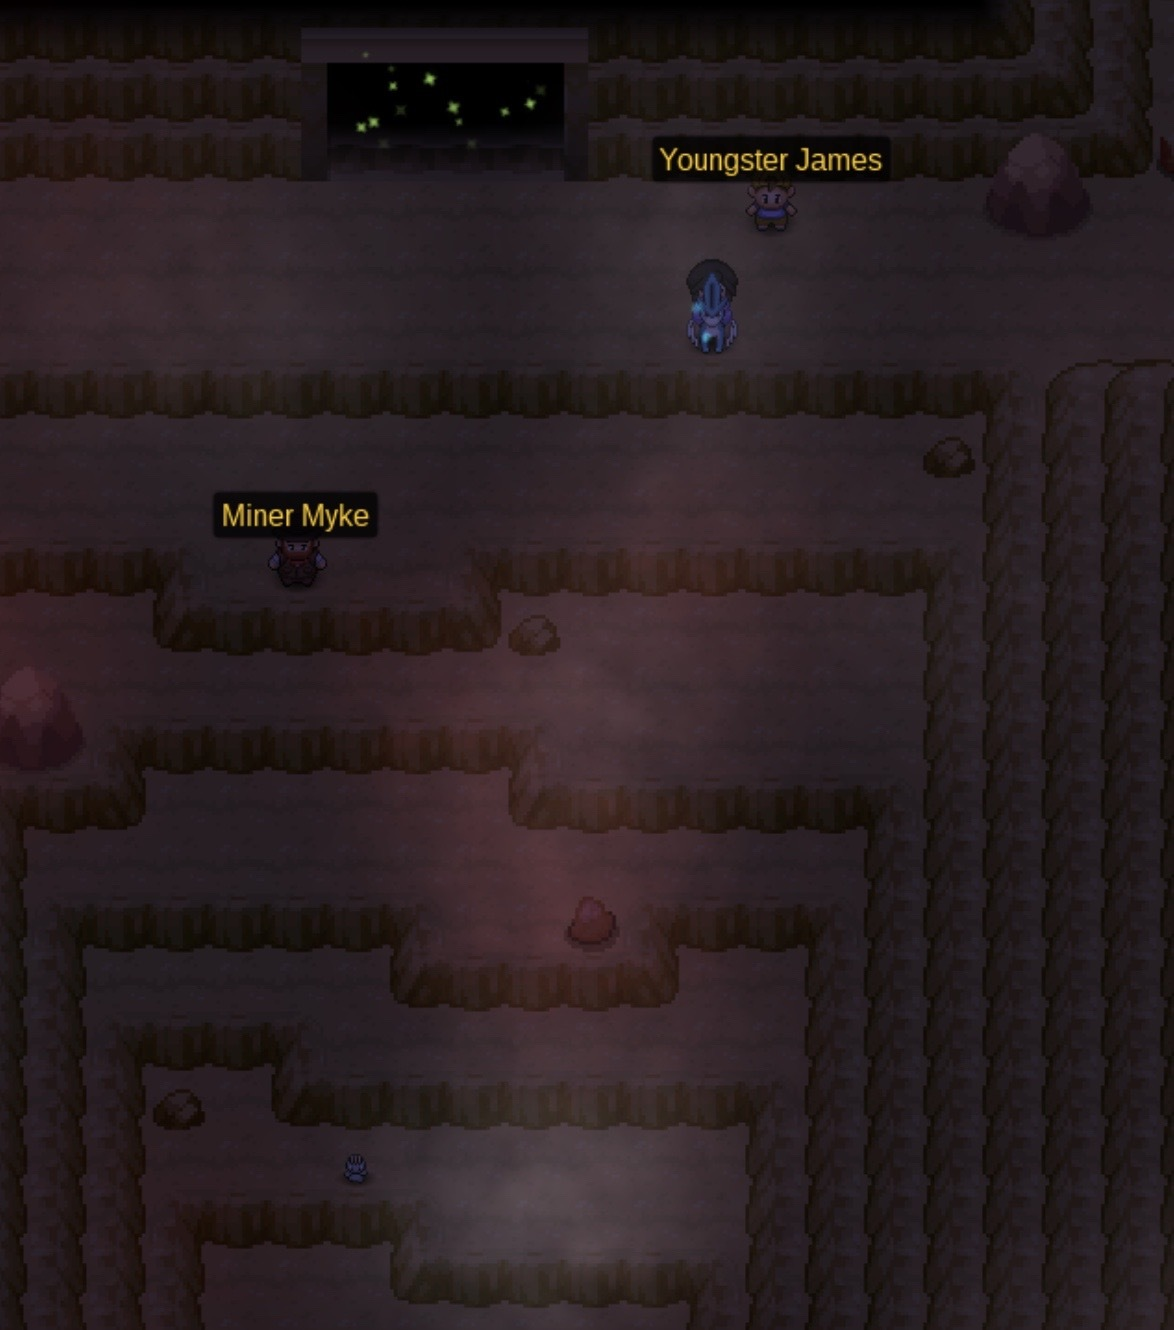
\includegraphics[width=\textwidth]{walkthrough/Sinnoh/oreburgh_mine}

\subsection{Oreburgh Gym}\label{subsec:oreburgh-gym}
Roark uses Rock-type pokemon.
After beating the gym go to Oreburgh City House 2 and you will find this NPC
selling rock smash, buy one we are going to need it later.

\section{Route 204}\label{sec:Route_204}

First head back to Jubilife City and talk with Looker and help him.
Now go to Route 204 and talk with the man in front of the cave enterence
in order to enter to the cave.

\subsection{Wild Pokemon}%
\label{subsec:WildPokemon}%
\begin{longtable}{||l l l l l l l l||}%
\hline%
Img&Pokémon&Level Range&Morning&Day&Night&Held Item&Rarity Tier\\%
\hline%
\endhead%
\hline%
&Bidoof&5{-}9&Morning&Day&Night&&Common\\%
\hline%
&Budew&5{-}9&Morning&Day&&&Uncommon\\%
\hline%
&Kricketot&5{-}9&Morning&Day&Night&&Uncommon\\%
\hline%
&Pineco&5{-}9&&Day&&&Rare\\%
\hline%
&Psyduck&5{-}9&Morning&&&&Common\\%
\hline%
&Seedot&5{-}9&Morning&Day&Night&&Common\\%
\hline%
&Shelmet&5{-}9&Morning&Day&Night&&Rare\\%
\hline%
&Shinx&5{-}9&Morning&Day&Night&&Rare\\%
\hline%
&Starly&5{-}9&Morning&Day&Night&&Common\\%
\hline%
&Sunkern&5{-}9&Morning&Day&&&Common\\%
\hline%
&Zubat&5{-}9&&&Night&&Common\\%
\hline%
\end{longtable}%
\begin{longtable}{||l l l l l l l l l||}%
\hline%
Img&Pokémon&Level Range&Morning&Day&Night&Rod&Held Item&Rarity Tier\\%
\hline%
\endhead%
\hline%
&Frillish&3{-}13&Morning&Day&Night&&&Rare\\%
\hline%
&Lombre&3{-}13&Morning&Day&Night&&&Uncommon\\%
\hline%
&Lotad&3{-}13&Morning&Day&Night&&&Uncommon\\%
\hline%
&Politoed&3{-}13&Morning&Day&Night&&&Rare\\%
\hline%
&Tentacool&3{-}13&Morning&Day&Night&&&Common\\%
\hline%
&Tentacruel&3{-}13&Morning&Day&Night&&&Common\\%
\hline%
\end{longtable}

\section{Ravaged Path}\label{sec:Ravaged_Path}

This is why we needed to buy rock smash, smash the rock and go to the next area.

\subsection{Wild Pokemon}%
\label{subsec:WildPokemon}%
\begin{longtable}{||l l l l l l l l||}%
\hline%
&Pokémon&Level Range&Morn&Day&Night&Held Item&Rarity Tier\\%
\hline%
\endhead%
\hline%
\includegraphics[width=0.02\textwidth]{pokemon/Geodude}&Geodude&3{-}7&Morn&Day&Night&&\textcolor{black}{%
Common%
}\\%
\hline%
\includegraphics[width=0.02\textwidth]{pokemon/Psyduck}&Psyduck&3{-}7&Morn&Day&Night&&\textcolor{black}{%
Common%
}\\%
\hline%
\includegraphics[width=0.02\textwidth]{pokemon/Zubat}&Zubat&3{-}7&Morn&Day&Night&&\textcolor{black}{%
Common%
}\\%
\hline%
\end{longtable}%
\caption{Ravaged Path Wild Pokemon (Land)}%
\begin{longtable}{||l l l l l l l l l||}%
\hline%
&Pokémon&Level Range&Morn&Day&Night&&Held Item&Rarity Tier\\%
\hline%
\endhead%
\hline%
\includegraphics[width=0.02\textwidth]{pokemon/Barboach}&Barboach&20{-}30&Morn&Day&Night&&&\textcolor{violet}{%
Rare%
}\\%
\hline%
\includegraphics[width=0.02\textwidth]{pokemon/Golduck}&Golduck&20{-}30&Morn&Day&Night&&&\textcolor{black}{%
Common%
}\\%
\hline%
\includegraphics[width=0.02\textwidth]{pokemon/Gyarados}&Gyarados&20{-}30&Morn&Day&Night&&&\textcolor{teal}{%
Uncommon%
}\\%
\hline%
\includegraphics[width=0.02\textwidth]{pokemon/Magikarp}&Magikarp&20{-}30&Morn&Day&Night&&&\textcolor{black}{%
Common%
}\\%
\hline%
\includegraphics[width=0.02\textwidth]{pokemon/Psyduck}&Psyduck&20{-}30&Morn&Day&Night&&&\textcolor{black}{%
Common%
}\\%
\hline%
\includegraphics[width=0.02\textwidth]{pokemon/Zubat}&Zubat&20{-}30&Morn&Day&Night&&&\textcolor{black}{%
Common%
}\\%
\hline%
\end{longtable}%
\caption{Ravaged Path Wild Pokemon (Water)}

\section{Valley Windworks}\label{sec:valley-windworks}

Finally we are in Floaroma town but skip that town and go to route 205,
we are going to meet Sandy and we need to help her dad.
Go to the right and we are going to find Galactic Team again, Beat him.
Now we need a password to enter, Go back to Floaroma Town.

\subsection{Wild Pokemon}%
\label{subsec:WildPokemon}%
\begin{longtable}{||l l l l l l l l||}%
\hline%
&Pokémon&Level Range&Morn&Day&Night&Held Item&Rarity Tier\\%
\hline%
\endhead%
\hline%
\includegraphics[width=0.02\textwidth]{pokemon/Buizel}&Buizel&11{-}14&Morn&Day&Night&&\textcolor{teal}{%
Uncommon%
}\\%
\hline%
\includegraphics[width=0.02\textwidth]{pokemon/Drifloon}&Drifloon&11{-}14&Morn&Day&Night&Air Balloon&\textcolor{violet}{%
Rare%
}\\%
\hline%
\includegraphics[width=0.02\textwidth]{pokemon/Elekid}&Elekid&11{-}14&&Day&&Electirizer&\textcolor{violet}{%
Rare%
}\\%
\hline%
\includegraphics[width=0.02\textwidth]{pokemon/Helioptile}&Helioptile&11{-}14&Morn&Day&Night&&\textcolor{violet}{%
Rare%
}\\%
\hline%
\includegraphics[width=0.02\textwidth]{pokemon/Mareep}&Mareep&11{-}14&Morn&Day&Night&&\textcolor{black}{%
Common%
}\\%
\hline%
\includegraphics[width=0.02\textwidth]{pokemon/Pachirisu}&Pachirisu&11{-}14&Morn&Day&Night&&\textcolor{violet}{%
Rare%
}\\%
\hline%
\includegraphics[width=0.02\textwidth]{pokemon/Shellos}&Shellos&11{-}14&Morn&Day&Night&&\textcolor{violet}{%
Rare%
}\\%
\hline%
\includegraphics[width=0.02\textwidth]{pokemon/Shinx}&Shinx&11{-}14&Morn&Day&Night&&\textcolor{violet}{%
Rare%
}\\%
\hline%
\includegraphics[width=0.02\textwidth]{pokemon/Starly}&Starly&11{-}14&Morn&Day&Night&&\textcolor{black}{%
Common%
}\\%
\hline%
\includegraphics[width=0.02\textwidth]{pokemon/Wingull}&Wingull&11{-}14&Morn&Day&Night&&\textcolor{black}{%
Common%
}\\%
\hline%
\end{longtable}%
\caption{Valley Windworks Wild Pokemon (Land)}%
\begin{longtable}{||l l l l l l l l l||}%
\hline%
&Pokémon&Level Range&Morn&Day&Night&&Held Item&Rarity Tier\\%
\hline%
\endhead%
\hline%
\includegraphics[width=0.02\textwidth]{pokemon/Finneon}&Finneon&20{-}35&Morn&Day&Night&&&\textcolor{teal}{%
Uncommon%
}\\%
\hline%
\includegraphics[width=0.02\textwidth]{pokemon/Gastrodon}&Gastrodon&20{-}35&Morn&Day&Night&&&\textcolor{violet}{%
Rare%
}\\%
\hline%
\includegraphics[width=0.02\textwidth]{pokemon/Gyarados}&Gyarados&20{-}35&Morn&Day&Night&&&\textcolor{teal}{%
Uncommon%
}\\%
\hline%
\includegraphics[width=0.02\textwidth]{pokemon/Magikarp}&Magikarp&20{-}35&Morn&Day&Night&&&\textcolor{black}{%
Common%
}\\%
\hline%
\includegraphics[width=0.02\textwidth]{pokemon/Pelipper}&Pelipper&20{-}35&Morn&Day&Night&&&\textcolor{teal}{%
Uncommon%
}\\%
\hline%
\includegraphics[width=0.02\textwidth]{pokemon/Shellder}&Shellder&20{-}35&Morn&Day&Night&&&\textcolor{teal}{%
Uncommon%
}\\%
\hline%
\includegraphics[width=0.02\textwidth]{pokemon/Shellos}&Shellos&20{-}35&Morn&Day&Night&&&\textcolor{violet}{%
Rare%
}\\%
\hline%
\includegraphics[width=0.02\textwidth]{pokemon/Tentacool}&Tentacool&20{-}35&Morn&Day&Night&&&\textcolor{black}{%
Common%
}\\%
\hline%
\includegraphics[width=0.02\textwidth]{pokemon/Tentacruel}&Tentacruel&20{-}35&Morn&Day&Night&&&\textcolor{teal}{%
Uncommon%
}\\%
\hline%
\includegraphics[width=0.02\textwidth]{pokemon/Wingull}&Wingull&20{-}35&Morn&Day&Night&&&\textcolor{black}{%
Common%
}\\%
\hline%
\end{longtable}%
\caption{Valley Windworks Wild Pokemon (Water)}

\section{Floaroma Town}\label{sec:floaroma-town}

Back in Floaroma Town, go to the top left area.
Beat the galactic guy and he is going to give us the password.
Go back to Valley Windworks and get ready to battle.

\section{Route 205}\label{sec:Route_205}

After you beat galactic guy, Go back to Route 205 and go to the north.
Nothing important in this route just a lot of trainers to get a lot of XP,
Go to the top and enter to Eterna Forest.

\subsection{Wild Pokemon}%
\label{subsec:WildPokemon}%
\begin{longtable}{||l l l l l l l l||}%
\hline%
&Pokémon&Level Range&Morn&Day&Night&Held Item&Rarity Tier\\%
\hline%
\endhead%
\hline%
\includegraphics[width=0.05\textwidth]{pokemon/Audino}&Audino&11{-}14&Morn&Day&Night&&\textcolor{violet}{%
Rare%
}\\%
\hline%
\includegraphics[width=0.05\textwidth]{pokemon/Bidoof}&Bidoof&11{-}14&Morn&Day&Night&&\textcolor{black}{%
Common%
}\\%
\hline%
\includegraphics[width=0.05\textwidth]{pokemon/Budew}&Budew&11{-}14&Morn&Day&&Hondew Berry&\textcolor{teal}{%
Uncommon%
}\\%
\hline%
\includegraphics[width=0.05\textwidth]{pokemon/Cascoon}&Cascoon&11{-}14&Morn&Day&Night&&\textcolor{teal}{%
Uncommon%
}\\%
\hline%
\includegraphics[width=0.05\textwidth]{pokemon/Cherrim}&Cherrim&11{-}14&Morn&Day&Night&Tamato Berry&\textcolor{teal}{%
Uncommon%
}\\%
\hline%
\includegraphics[width=0.05\textwidth]{pokemon/Combee}&Combee&11{-}14&Morn&Day&Night&Honey&\textcolor{teal}{%
Uncommon%
}\\%
\hline%
\includegraphics[width=0.05\textwidth]{pokemon/Dustox}&Dustox&11{-}14&Morn&Day&Night&&\textcolor{teal}{%
Uncommon%
}\\%
\hline%
\includegraphics[width=0.05\textwidth]{pokemon/Espurr}&Espurr&20{-}23&Morn&Day&&&\textcolor{violet}{%
Rare%
}\\%
\hline%
\includegraphics[width=0.05\textwidth]{pokemon/Hoothoot}&Hoothoot&11{-}14&&&Night&&\textcolor{black}{%
Common%
}\\%
\hline%
\includegraphics[width=0.05\textwidth]{pokemon/Misdreavus}&Misdreavus&11{-}14&&&Night&&\textcolor{teal}{%
Uncommon%
}\\%
\hline%
\includegraphics[width=0.05\textwidth]{pokemon/Murkrow}&Murkrow&11{-}14&&&Night&&\textcolor{violet}{%
Rare%
}\\%
\hline%
\includegraphics[width=0.05\textwidth]{pokemon/Silcoon}&Silcoon&11{-}14&Morn&Day&Night&&\textcolor{teal}{%
Uncommon%
}\\%
\hline%
\includegraphics[width=0.05\textwidth]{pokemon/Wurmple}&Wurmple&11{-}14&Morn&Day&Night&&\textcolor{black}{%
Common%
}\\%
\hline%
\end{longtable}%
\caption{Route 205 Wild Pokemon (Land)}%
\begin{longtable}{||l l l l l l l l l||}%
\hline%
&Pokémon&Level Range&Morn&Day&Night&&Held Item&Rarity Tier\\%
\hline%
\endhead%
\hline%
\includegraphics[width=0.05\textwidth]{pokemon/Bidoof}&Bidoof&11{-}14&Morn&Day&Night&&&\textcolor{black}{%
Common%
}\\%
\hline%
\includegraphics[width=0.05\textwidth]{pokemon/Buizel}&Buizel&11{-}14&Morn&Day&Night&&&\textcolor{teal}{%
Uncommon%
}\\%
\hline%
\includegraphics[width=0.05\textwidth]{pokemon/Golduck}&Golduck&14{-}17&Morn&Day&Night&&&\textcolor{black}{%
Common%
}\\%
\hline%
\includegraphics[width=0.05\textwidth]{pokemon/Magikarp}&Magikarp&11{-}14&Morn&Day&Night&&&\textcolor{black}{%
Common%
}\\%
\hline%
\includegraphics[width=0.05\textwidth]{pokemon/Psyduck}&Psyduck&11{-}14&Morn&Day&Night&&&\textcolor{black}{%
Common%
}\\%
\hline%
\end{longtable}%
\caption{Route 205 Wild Pokemon (Water)}

\section{Eterna Forest}\label{sec:Eterna_Forest}

Eterna forest have a lot of trainers as well.
After you beat them all go to the top right and you are in the second area of route 205.

\subsection{Wild Pokemon}%
\label{subsec:WildPokemon}%
\begin{longtable}{||l l l l l l l l||}%
\hline%
&Pokémon&Level Range&Morn&Day&Night&Held Item&Rarity Tier\\%
\hline%
\endhead%
\hline%
\includegraphics[width=0.05\textwidth]{pokemon/Buneary}&Buneary&15{-}18&Morn&Day&&&\textcolor{violet}{%
Rare%
}\\%
\hline%
\includegraphics[width=0.05\textwidth]{pokemon/Cascoon}&Cascoon&11{-}14&Morn&Day&Night&&\textcolor{teal}{%
Uncommon%
}\\%
\hline%
\includegraphics[width=0.05\textwidth]{pokemon/Cherrim}&Cherrim&11{-}14&Morn&Day&Night&Tamato Berry&\textcolor{teal}{%
Uncommon%
}\\%
\hline%
\includegraphics[width=0.05\textwidth]{pokemon/Dustox}&Dustox&11{-}14&Morn&Day&Night&&\textcolor{teal}{%
Uncommon%
}\\%
\hline%
\includegraphics[width=0.05\textwidth]{pokemon/Hoothoot}&Hoothoot&11{-}14&&&Night&&\textcolor{black}{%
Common%
}\\%
\hline%
\includegraphics[width=0.05\textwidth]{pokemon/Karrablast}&Karrablast&11{-}14&Morn&Day&Night&&\textcolor{violet}{%
Rare%
}\\%
\hline%
\includegraphics[width=0.05\textwidth]{pokemon/Misdreavus}&Misdreavus&11{-}14&&&Night&&\textcolor{teal}{%
Uncommon%
}\\%
\hline%
\includegraphics[width=0.05\textwidth]{pokemon/Murkrow}&Murkrow&11{-}14&&&Night&&\textcolor{violet}{%
Rare%
}\\%
\hline%
\includegraphics[width=0.05\textwidth]{pokemon/Silcoon}&Silcoon&11{-}14&Morn&Day&Night&&\textcolor{teal}{%
Uncommon%
}\\%
\hline%
\includegraphics[width=0.05\textwidth]{pokemon/Starly}&Starly&11{-}14&Morn&Day&Night&&\textcolor{black}{%
Common%
}\\%
\hline%
\includegraphics[width=0.05\textwidth]{pokemon/Whirlipede}&Whirlipede&11{-}14&Morn&Day&Night&&\textcolor{violet}{%
Rare%
}\\%
\hline%
\end{longtable}%
\caption{Eterna Forest Wild Pokemon (Land)}

\section{Eterna City}\label{sec:eterna-city}
Now we are in Eterna City.
Go to the gym and you are going to find Gardenia outside and she will ask you
if you can check the building in the north of the city.
Go to the building and we are going to find grunts for Galactic Team again.
Be ready to battle.
Once in the building go to the top and you will find
Commander Jupiter and Jevons, Talk with Jupiter and beat him.
After you beat him talk with Devons and help him to find some pokemon.
Pokemon Locations:

After you find all pokemons, Talk with Jevons again and then go to the gym.

\subsection{Eterna City Gym}\label{subsec:eterna-city-gym}
Gardenia uses Grass-type Pokemon.
Beat her and get the badge.

\section{Route 211 (West)}\label{sec:Route_211_(West)}

\subsection{Wild Pokemon}%
\label{subsec:WildPokemon}%
\begin{longtable}{||l l l l l l l l||}%
\hline%
&Pokémon&Level Range&Morn&Day&Night&Held Item&Rarity Tier\\%
\hline%
\endhead%
\hline%
\includegraphics[width=0.05\textwidth]{pokemon/Bidoof}&Bidoof&13{-}17&Morn&Day&Night&&\textcolor{black}{%
Common%
}\\%
\hline%
\includegraphics[width=0.05\textwidth]{pokemon/Bronzor}&Bronzor&13{-}17&Morn&Day&Night&&\textcolor{teal}{%
Uncommon%
}\\%
\hline%
\includegraphics[width=0.05\textwidth]{pokemon/Cherubi}&Cherubi&13{-}17&Morn&Day&Night&&\textcolor{black}{%
Common%
}\\%
\hline%
\includegraphics[width=0.05\textwidth]{pokemon/Chingling}&Chingling&13{-}17&Morn&Day&Night&&\textcolor{teal}{%
Uncommon%
}\\%
\hline%
\includegraphics[width=0.05\textwidth]{pokemon/Chingling}&Chingling&13{-}17&Morn&Day&Night&&\textcolor{teal}{%
Uncommon%
}\\%
\hline%
\includegraphics[width=0.05\textwidth]{pokemon/Hoothoot}&Hoothoot&13{-}17&&&Night&&\textcolor{black}{%
Common%
}\\%
\hline%
\includegraphics[width=0.05\textwidth]{pokemon/Machop}&Machop&13{-}17&Morn&Day&Night&&\textcolor{black}{%
Common%
}\\%
\hline%
\includegraphics[width=0.05\textwidth]{pokemon/Meditite}&Meditite&13{-}17&Morn&Day&Night&&\textcolor{violet}{%
Rare%
}\\%
\hline%
\includegraphics[width=0.05\textwidth]{pokemon/Ponyta}&Ponyta&13{-}17&Morn&Day&Night&&\textcolor{teal}{%
Uncommon%
}\\%
\hline%
\includegraphics[width=0.05\textwidth]{pokemon/Skiddo}&Skiddo&13{-}17&Morn&Day&Night&&\textcolor{violet}{%
Rare%
}\\%
\hline%
\includegraphics[width=0.05\textwidth]{pokemon/Swablu}&Swablu&13{-}17&&Day&&&\textcolor{violet}{%
Rare%
}\\%
\hline%
\includegraphics[width=0.05\textwidth]{pokemon/Zubat}&Zubat&13{-}17&&&Night&&\textcolor{black}{%
Common%
}\\%
\hline%
\end{longtable}%
\caption{Route 211 Wild Pokemon (Land)}

\section{Mt. Coronet (Northern Area Part 1)}
\label{sec:Mt._Coronet}
\subsection{Wild Pokemon}%
\label{subsec:WildPokemon}%


\section{Old Chateau}
\label{sec:Old_Chateau}
\subsection{Wild Pokemon}%
\label{subsec:WildPokemon}%
\begin{longtable}{||l l l l l l l l||}%
\hline%
&Pokémon&Level Range&Morn&Day&Night&Held Item&Rarity Tier\\%
\hline%
\endhead%
\hline%
\includegraphics[width=0.05\textwidth]{pokemon/Drowzee}&Drowzee&11{-}14&Morn&Day&&&\textcolor{black}{%
Common%
}\\%
\hline%
\includegraphics[width=0.05\textwidth]{pokemon/Espurr}&Espurr&20{-}22&Morn&Day&Night&&\textcolor{violet}{%
Rare%
}\\%
\hline%
\includegraphics[width=0.05\textwidth]{pokemon/Gastly}&Gastly&11{-}14&Morn&Day&Night&&\textcolor{teal}{%
Uncommon%
}\\%
\hline%
\includegraphics[width=0.05\textwidth]{pokemon/Golbat}&Golbat&11{-}14&Morn&Day&Night&&\textcolor{black}{%
Common%
}\\%
\hline%
\includegraphics[width=0.05\textwidth]{pokemon/Haunter}&Haunter&11{-}14&Morn&Day&Night&&\textcolor{teal}{%
Uncommon%
}\\%
\hline%
\includegraphics[width=0.05\textwidth]{pokemon/Patrat}&Patrat&11{-}14&Morn&Day&Night&&\textcolor{black}{%
Common%
}\\%
\hline%
\includegraphics[width=0.05\textwidth]{pokemon/Unown}&Unown&11{-}14&Morn&Day&Night&&\textcolor{black}{%
Common%
}\\%
\hline%
\includegraphics[width=0.05\textwidth]{pokemon/Zubat}&Zubat&11{-}14&Morn&Day&Night&&\textcolor{black}{%
Common%
}\\%
\hline%
\end{longtable}%
\caption{Old Chateau Wild Pokemon (Land)}%
\begin{longtable}{||l l l l l l l l||}%
\hline%
&Pokémon&Level Range&Morn&Day&Night&Held Item&Rarity Tier\\%
\hline%
\endhead%
\hline%
\includegraphics[width=0.05\textwidth]{pokemon/Abra}&Abra&11{-}15&Morn&Day&Night&&\textcolor{teal}{%
Uncommon%
}\\%
\hline%
\includegraphics[width=0.05\textwidth]{pokemon/Drowzee}&Drowzee&11{-}15&Morn&Day&Night&&\textcolor{black}{%
Common%
}\\%
\hline%
\includegraphics[width=0.05\textwidth]{pokemon/Gastly}&Gastly&11{-}15&Morn&Day&Night&&\textcolor{black}{%
Common%
}\\%
\hline%
\includegraphics[width=0.05\textwidth]{pokemon/Haunter}&Haunter&11{-}15&Morn&Day&Night&&\textcolor{teal}{%
Uncommon%
}\\%
\hline%
\includegraphics[width=0.05\textwidth]{pokemon/Kadabra}&Kadabra&16{-}20&Morn&Day&Night&&\textcolor{violet}{%
Rare%
}\\%
\hline%
\includegraphics[width=0.05\textwidth]{pokemon/Misdreavus}&Misdreavus&11{-}15&Morn&Day&Night&&\textcolor{teal}{%
Uncommon%
}\\%
\hline%
\includegraphics[width=0.05\textwidth]{pokemon/Murkrow}&Murkrow&11{-}15&Morn&Day&Night&&\textcolor{violet}{%
Rare%
}\\%
\hline%
\includegraphics[width=0.05\textwidth]{pokemon/Raticate}&Raticate&11{-}15&Morn&Day&Night&&\textcolor{black}{%
Common%
}\\%
\hline%
\includegraphics[width=0.05\textwidth]{pokemon/Rattata}&Rattata&11{-}15&Morn&Day&Night&&\textcolor{black}{%
Common%
}\\%
\hline%
\includegraphics[width=0.05\textwidth]{pokemon/Spiritomb}&Spiritomb&16{-}20&Morn&Day&Night&&\textcolor{violet}{%
Rare%
}\\%
\hline%
\end{longtable}%
\caption{Old Chateau Wild Pokemon (Land)}%
\begin{longtable}{||l l l l l l l l||}%
\hline%
&Pokémon&Level Range&Morn&Day&Night&Held Item&Rarity Tier\\%
\hline%
\endhead%
\hline%
\end{longtable}%
\caption{Old Chateau Wild Pokemon (Land)}%
\begin{longtable}{||l l l l l l l l||}%
\hline%
&Pokémon&Level Range&Morn&Day&Night&Held Item&Rarity Tier\\%
\hline%
\endhead%
\hline%
\includegraphics[width=0.05\textwidth]{pokemon/Gastly}&Gastly&11{-}14&Morn&Day&&&\textcolor{black}{%
Common%
}\\%
\hline%
\includegraphics[width=0.05\textwidth]{pokemon/Gengar}&Gengar&11{-}14&Morn&Day&&&\textcolor{violet}{%
Rare%
}\\%
\hline%
\includegraphics[width=0.05\textwidth]{pokemon/Golbat}&Golbat&11{-}14&Morn&Day&&&\textcolor{black}{%
Common%
}\\%
\hline%
\includegraphics[width=0.05\textwidth]{pokemon/Haunter}&Haunter&11{-}14&Morn&Day&&&\textcolor{teal}{%
Uncommon%
}\\%
\hline%
\includegraphics[width=0.05\textwidth]{pokemon/Misdreavus}&Misdreavus&11{-}14&Morn&Day&&&\textcolor{teal}{%
Uncommon%
}\\%
\hline%
\includegraphics[width=0.05\textwidth]{pokemon/Patrat}&Patrat&11{-}14&Morn&Day&&&\textcolor{black}{%
Common%
}\\%
\hline%
\includegraphics[width=0.05\textwidth]{pokemon/Rattata}&Rattata&11{-}14&Morn&Day&&&\textcolor{black}{%
Common%
}\\%
\hline%
\includegraphics[width=0.05\textwidth]{pokemon/Zubat}&Zubat&11{-}14&Morn&Day&&&\textcolor{black}{%
Common%
}\\%
\hline%
\end{longtable}%
\caption{Old Chateau Wild Pokemon (Land)}%
\begin{longtable}{||l l l l l l l l||}%
\hline%
&Pokémon&Level Range&Morn&Day&Night&Held Item&Rarity Tier\\%
\hline%
\endhead%
\hline%
\includegraphics[width=0.05\textwidth]{pokemon/Gastly}&Gastly&11{-}14&Morn&Day&&&\textcolor{black}{%
Common%
}\\%
\hline%
\includegraphics[width=0.05\textwidth]{pokemon/Gengar}&Gengar&11{-}14&Morn&Day&&&\textcolor{violet}{%
Rare%
}\\%
\hline%
\includegraphics[width=0.05\textwidth]{pokemon/Golbat}&Golbat&11{-}14&Morn&Day&&&\textcolor{black}{%
Common%
}\\%
\hline%
\includegraphics[width=0.05\textwidth]{pokemon/Haunter}&Haunter&11{-}14&Morn&Day&&&\textcolor{teal}{%
Uncommon%
}\\%
\hline%
\includegraphics[width=0.05\textwidth]{pokemon/Misdreavus}&Misdreavus&11{-}14&Morn&Day&&&\textcolor{teal}{%
Uncommon%
}\\%
\hline%
\includegraphics[width=0.05\textwidth]{pokemon/Patrat}&Patrat&11{-}14&Morn&Day&&&\textcolor{black}{%
Common%
}\\%
\hline%
\includegraphics[width=0.05\textwidth]{pokemon/Rattata}&Rattata&11{-}14&Morn&Day&&&\textcolor{black}{%
Common%
}\\%
\hline%
\includegraphics[width=0.05\textwidth]{pokemon/Zubat}&Zubat&11{-}14&Morn&Day&&&\textcolor{black}{%
Common%
}\\%
\hline%
\end{longtable}%
\caption{Old Chateau Wild Pokemon (Land)}%
\begin{longtable}{||l l l l l l l l||}%
\hline%
&Pokémon&Level Range&Morn&Day&Night&Held Item&Rarity Tier\\%
\hline%
\endhead%
\hline%
\includegraphics[width=0.05\textwidth]{pokemon/Gastly}&Gastly&11{-}14&Morn&Day&&&\textcolor{black}{%
Common%
}\\%
\hline%
\includegraphics[width=0.05\textwidth]{pokemon/Gengar}&Gengar&11{-}14&Morn&Day&&&\textcolor{violet}{%
Rare%
}\\%
\hline%
\includegraphics[width=0.05\textwidth]{pokemon/Golbat}&Golbat&11{-}14&Morn&Day&&&\textcolor{black}{%
Common%
}\\%
\hline%
\includegraphics[width=0.05\textwidth]{pokemon/Haunter}&Haunter&11{-}14&Morn&Day&&&\textcolor{teal}{%
Uncommon%
}\\%
\hline%
\includegraphics[width=0.05\textwidth]{pokemon/Misdreavus}&Misdreavus&11{-}14&Morn&Day&&&\textcolor{teal}{%
Uncommon%
}\\%
\hline%
\includegraphics[width=0.05\textwidth]{pokemon/Patrat}&Patrat&11{-}14&Morn&Day&&&\textcolor{black}{%
Common%
}\\%
\hline%
\includegraphics[width=0.05\textwidth]{pokemon/Rattata}&Rattata&11{-}14&Morn&Day&&&\textcolor{black}{%
Common%
}\\%
\hline%
\includegraphics[width=0.05\textwidth]{pokemon/Zubat}&Zubat&11{-}14&Morn&Day&&&\textcolor{black}{%
Common%
}\\%
\hline%
\end{longtable}%
\caption{Old Chateau Wild Pokemon (Land)}%
\begin{longtable}{||l l l l l l l l||}%
\hline%
&Pokémon&Level Range&Morn&Day&Night&Held Item&Rarity Tier\\%
\hline%
\endhead%
\hline%
\includegraphics[width=0.05\textwidth]{pokemon/Gastly}&Gastly&11{-}14&Morn&Day&&&\textcolor{black}{%
Common%
}\\%
\hline%
\includegraphics[width=0.05\textwidth]{pokemon/Gengar}&Gengar&11{-}14&Morn&Day&&&\textcolor{violet}{%
Rare%
}\\%
\hline%
\includegraphics[width=0.05\textwidth]{pokemon/Golbat}&Golbat&11{-}14&Morn&Day&&&\textcolor{black}{%
Common%
}\\%
\hline%
\includegraphics[width=0.05\textwidth]{pokemon/Haunter}&Haunter&11{-}14&Morn&Day&&&\textcolor{teal}{%
Uncommon%
}\\%
\hline%
\includegraphics[width=0.05\textwidth]{pokemon/Misdreavus}&Misdreavus&11{-}14&Morn&Day&&&\textcolor{teal}{%
Uncommon%
}\\%
\hline%
\includegraphics[width=0.05\textwidth]{pokemon/Patrat}&Patrat&11{-}14&Morn&Day&&&\textcolor{black}{%
Common%
}\\%
\hline%
\includegraphics[width=0.05\textwidth]{pokemon/Rattata}&Rattata&11{-}14&Morn&Day&&&\textcolor{black}{%
Common%
}\\%
\hline%
\includegraphics[width=0.05\textwidth]{pokemon/Zubat}&Zubat&11{-}14&Morn&Day&&&\textcolor{black}{%
Common%
}\\%
\hline%
\end{longtable}%
\caption{Old Chateau Wild Pokemon (Land)}%
\begin{longtable}{||l l l l l l l l||}%
\hline%
&Pokémon&Level Range&Morn&Day&Night&Held Item&Rarity Tier\\%
\hline%
\endhead%
\hline%
\includegraphics[width=0.05\textwidth]{pokemon/Gastly}&Gastly&11{-}14&Morn&Day&&&\textcolor{black}{%
Common%
}\\%
\hline%
\includegraphics[width=0.05\textwidth]{pokemon/Gengar}&Gengar&11{-}14&Morn&Day&&&\textcolor{violet}{%
Rare%
}\\%
\hline%
\includegraphics[width=0.05\textwidth]{pokemon/Golbat}&Golbat&11{-}14&Morn&Day&&&\textcolor{black}{%
Common%
}\\%
\hline%
\includegraphics[width=0.05\textwidth]{pokemon/Haunter}&Haunter&11{-}14&Morn&Day&&&\textcolor{teal}{%
Uncommon%
}\\%
\hline%
\includegraphics[width=0.05\textwidth]{pokemon/Misdreavus}&Misdreavus&11{-}14&Morn&Day&&&\textcolor{teal}{%
Uncommon%
}\\%
\hline%
\includegraphics[width=0.05\textwidth]{pokemon/Patrat}&Patrat&11{-}14&Morn&Day&&&\textcolor{black}{%
Common%
}\\%
\hline%
\includegraphics[width=0.05\textwidth]{pokemon/Rattata}&Rattata&11{-}14&Morn&Day&&&\textcolor{black}{%
Common%
}\\%
\hline%
\includegraphics[width=0.05\textwidth]{pokemon/Zubat}&Zubat&11{-}14&Morn&Day&&&\textcolor{black}{%
Common%
}\\%
\hline%
\end{longtable}%
\caption{Old Chateau Wild Pokemon (Land)}%
\begin{longtable}{||l l l l l l l l||}%
\hline%
&Pokémon&Level Range&Morn&Day&Night&Held Item&Rarity Tier\\%
\hline%
\endhead%
\hline%
\includegraphics[width=0.05\textwidth]{pokemon/Gastly}&Gastly&11{-}14&Morn&Day&&&\textcolor{black}{%
Common%
}\\%
\hline%
\includegraphics[width=0.05\textwidth]{pokemon/Gengar}&Gengar&11{-}14&Morn&Day&&&\textcolor{violet}{%
Rare%
}\\%
\hline%
\includegraphics[width=0.05\textwidth]{pokemon/Golbat}&Golbat&11{-}14&Morn&Day&&&\textcolor{black}{%
Common%
}\\%
\hline%
\includegraphics[width=0.05\textwidth]{pokemon/Haunter}&Haunter&11{-}14&Morn&Day&&&\textcolor{teal}{%
Uncommon%
}\\%
\hline%
\includegraphics[width=0.05\textwidth]{pokemon/Misdreavus}&Misdreavus&11{-}14&Morn&Day&&&\textcolor{teal}{%
Uncommon%
}\\%
\hline%
\includegraphics[width=0.05\textwidth]{pokemon/Patrat}&Patrat&11{-}14&Morn&Day&&&\textcolor{black}{%
Common%
}\\%
\hline%
\includegraphics[width=0.05\textwidth]{pokemon/Rattata}&Rattata&11{-}14&Morn&Day&&&\textcolor{black}{%
Common%
}\\%
\hline%
\includegraphics[width=0.05\textwidth]{pokemon/Zubat}&Zubat&11{-}14&Morn&Day&&&\textcolor{black}{%
Common%
}\\%
\hline%
\end{longtable}%
\caption{Old Chateau Wild Pokemon (Land)}%
\begin{longtable}{||l l l l l l l l||}%
\hline%
&Pokémon&Level Range&Morn&Day&Night&Held Item&Rarity Tier\\%
\hline%
\endhead%
\hline%
\includegraphics[width=0.05\textwidth]{pokemon/Gastly}&Gastly&11{-}14&Morn&Day&&&\textcolor{black}{%
Common%
}\\%
\hline%
\includegraphics[width=0.05\textwidth]{pokemon/Gengar}&Gengar&11{-}14&Morn&Day&&&\textcolor{violet}{%
Rare%
}\\%
\hline%
\includegraphics[width=0.05\textwidth]{pokemon/Golbat}&Golbat&11{-}14&Morn&Day&&&\textcolor{black}{%
Common%
}\\%
\hline%
\includegraphics[width=0.05\textwidth]{pokemon/Haunter}&Haunter&11{-}14&Morn&Day&&&\textcolor{teal}{%
Uncommon%
}\\%
\hline%
\includegraphics[width=0.05\textwidth]{pokemon/Misdreavus}&Misdreavus&11{-}14&Morn&Day&&&\textcolor{teal}{%
Uncommon%
}\\%
\hline%
\includegraphics[width=0.05\textwidth]{pokemon/Patrat}&Patrat&11{-}14&Morn&Day&&&\textcolor{black}{%
Common%
}\\%
\hline%
\includegraphics[width=0.05\textwidth]{pokemon/Rattata}&Rattata&11{-}14&Morn&Day&&&\textcolor{black}{%
Common%
}\\%
\hline%
\includegraphics[width=0.05\textwidth]{pokemon/Zubat}&Zubat&11{-}14&Morn&Day&&&\textcolor{black}{%
Common%
}\\%
\hline%
\end{longtable}%
\caption{Old Chateau Wild Pokemon (Land)}

\section{Route 206}\label{sec:Route_206}

Nothing important in this routes just beat all the trainers to get Xp.

\subsection{Wild Pokemon}%
\label{subsec:WildPokemon}%
\begin{longtable}{||l l l l l l l l||}%
\hline%
&Pokémon&Level Range&Morn&Day&Night&Held Item&Rarity Tier\\%
\hline%
\endhead%
\hline%
\includegraphics[width=0.02\textwidth]{pokemon/Blitzle}&Blitzle&15{-}19&Morn&&Night&Cheri Berry&\textcolor{violet}{%
Rare%
}\\%
\hline%
\includegraphics[width=0.02\textwidth]{pokemon/Bronzor}&Bronzor&15{-}19&Morn&Day&Night&&\textcolor{teal}{%
Uncommon%
}\\%
\hline%
\includegraphics[width=0.02\textwidth]{pokemon/Geodude}&Geodude&15{-}19&&Day&&&\textcolor{black}{%
Common%
}\\%
\hline%
\includegraphics[width=0.02\textwidth]{pokemon/Kricketot}&Kricketot&15{-}19&Morn&Day&Night&&\textcolor{teal}{%
Uncommon%
}\\%
\hline%
\includegraphics[width=0.02\textwidth]{pokemon/Kricketune}&Kricketune&15{-}19&Morn&Day&Night&&\textcolor{teal}{%
Uncommon%
}\\%
\hline%
\includegraphics[width=0.02\textwidth]{pokemon/Larvitar}&Larvitar&15{-}19&Morn&Day&Night&&\textcolor{violet}{%
Rare%
}\\%
\hline%
\includegraphics[width=0.02\textwidth]{pokemon/Machop}&Machop&15{-}19&Morn&Day&Night&&\textcolor{black}{%
Common%
}\\%
\hline%
\includegraphics[width=0.02\textwidth]{pokemon/Ponyta}&Ponyta&15{-}19&Morn&Day&Night&&\textcolor{teal}{%
Uncommon%
}\\%
\hline%
\includegraphics[width=0.02\textwidth]{pokemon/Stunky}&Stunky&15{-}19&Morn&Day&Night&&\textcolor{teal}{%
Uncommon%
}\\%
\hline%
\includegraphics[width=0.02\textwidth]{pokemon/Zubat}&Zubat&15{-}19&Morn&&Night&&\textcolor{black}{%
Common%
}\\%
\hline%
\end{longtable}%
\caption{Route 206 Wild Pokemon (Land)}

\section{Wayward Cave}
\label{sec:Wayward_Cave}
\subsection{Wild Pokemon}%
\label{subsec:WildPokemon}%
\begin{longtable}{||l l l l l l l l||}%
\hline%
&Pokémon&Level Range&Morn&Day&Night&Held Item&Rarity Tier\\%
\hline%
\endhead%
\hline%
\includegraphics[width=0.05\textwidth]{pokemon/Bronzor}&Bronzor&15{-}19&Morn&Day&Night&&\textcolor{teal}{%
Uncommon%
}\\%
\hline%
\includegraphics[width=0.05\textwidth]{pokemon/Bunnelby}&Bunnelby&20{-}30&Morn&Day&Night&&\textcolor{violet}{%
Rare%
}\\%
\hline%
\includegraphics[width=0.05\textwidth]{pokemon/Gible}&Gible&5{-}14&Morn&&Night&&\textcolor{violet}{%
Rare%
}\\%
\hline%
\includegraphics[width=0.05\textwidth]{pokemon/Onix}&Onix&15{-}19&Morn&Day&Night&&\textcolor{teal}{%
Uncommon%
}\\%
\hline%
\includegraphics[width=0.05\textwidth]{pokemon/Sandshrew}&Sandshrew&15{-}19&Morn&Day&Night&&\textcolor{black}{%
Common%
}\\%
\hline%
\includegraphics[width=0.05\textwidth]{pokemon/Zubat}&Zubat&15{-}19&Morn&Day&Night&&\textcolor{black}{%
Common%
}\\%
\hline%
\end{longtable}%
\caption{Wayward Cave Wild Pokemon (Land)}

\section{Route 207}\label{sec:Route_207}

In the cave from route 207 you will find Cyrus but you are not going to have a battle.

\subsubsection{Wild Pokémon}%
\label{ssubsec:WildPokmon}%
\begin{longtable}{||l l l l l l l l||}%
\hline%
\rowcolor{GroundColor}%
&Pokémon&Level Range&Morn&Day&Night&Held Item&Rarity Tier\\%
\hline%
\endhead%
\hline%
\rowcolor{GroundColor}%
\includegraphics[width=0.02\textwidth]{pokemon/Burmy}&Burmy&6{-}9&Morn&Day&Night&&\textcolor{OliveGreen}{%
Uncommon%
}\\%
\hline%
\rowcolor{GroundColor}%
\includegraphics[width=0.02\textwidth]{pokemon/Geodude}&Geodude&6{-}9&Morn&Day&Night&Everstone&\textcolor{black}{%
Common%
}\\%
\hline%
\rowcolor{GroundColor}%
\includegraphics[width=0.02\textwidth]{pokemon/Gligar}&Gligar&6{-}9&&&Night&&\textcolor{RedOrange}{%
Rare%
}\\%
\hline%
\rowcolor{GroundColor}%
\includegraphics[width=0.02\textwidth]{pokemon/Kricketot}&Kricketot&6{-}9&Morn&Day&Night&&\textcolor{OliveGreen}{%
Uncommon%
}\\%
\hline%
\rowcolor{GroundColor}%
\includegraphics[width=0.02\textwidth]{pokemon/Machop}&Machop&6{-}9&Morn&Day&Night&&\textcolor{black}{%
Common%
}\\%
\hline%
\rowcolor{GroundColor}%
\includegraphics[width=0.02\textwidth]{pokemon/Phanpy}&Phanpy&6{-}9&Morn&Day&Night&&\textcolor{OliveGreen}{%
Uncommon%
}\\%
\hline%
\rowcolor{GroundColor}%
\includegraphics[width=0.02\textwidth]{pokemon/Ponyta}&Ponyta&6{-}9&Morn&Day&Night&&\textcolor{OliveGreen}{%
Uncommon%
}\\%
\hline%
\rowcolor{GroundColor}%
\includegraphics[width=0.02\textwidth]{pokemon/Zubat}&Zubat&6{-}9&&&Night&&\textcolor{black}{%
Common%
}\\%
\hline%
\end{longtable}%
\caption{Wild Pokemon in Route 207}


\begin{mdframed}[style=MyFrame,nobreak=true,frametitle={Pokemon Spotlight: Gligar}]

\begin{wrapfigure}{l}{0.33\textwidth}
\includegraphics[width=0.33\textwidth]{walkthrough/Sinnoh/spotlight-gligar}
\label{fig:spotlight-gligar}
\end{wrapfigure}

Gligar's Hidden Ability, Poison Heal, allows it to be immune to status effects
when poisoned while also providing it with passive recovery, which is useful
alongside reliable recovery in Roost.
Using a Toxic Orb allows the poison to be applied automatically.

Gligar evolves into Gliscor when leveled up holding a Razor Fang during the night.
Find one with a Careful nature with high IVs in HP, Special Defense, and Speed.

If you don't want to grind for a Gligar with Poison Heal, a viable build can
also be made using Hyper Cutter.
Jolly or Impish Nature can also work.

\end{mdframed}

\section{Route 208}\label{sec:Route_208}
\subsection{Wild Pokemon}%
\label{subsec:WildPokemon}%
\begin{longtable}{||l l l l l l l l||}%
\hline%
Img&Pokémon&Level Range&Morning&Day&Night&Held Item&Rarity Tier\\%
\hline%
\endhead%
\hline%
&Dunsparce&17{-}22&Morning&&&&Common\\%
\hline%
&Gastly&17{-}22&&Day&&&Common\\%
\hline%
&Gengar&17{-}22&&Day&&&Uncommon\\%
\hline%
&Haunter&17{-}22&&Day&&&Uncommon\\%
\hline%
&Kricketune&17{-}22&&&Night&&Uncommon\\%
\hline%
&Lickilicky&17{-}22&Morning&&&&Uncommon\\%
\hline%
&Lickitung&17{-}22&Morning&&&&Uncommon\\%
\hline%
&Patrat&17{-}22&&&Night&&Common\\%
\hline%
&Staraptor&17{-}22&&&Night&&Uncommon\\%
\hline%
\end{longtable}%
\begin{longtable}{||l l l l l l l l l||}%
\hline%
Img&Pokémon&Level Range&Morning&Day&Night&Rod&Held Item&Rarity Tier\\%
\hline%
\endhead%
\hline%
&Crobat&17{-}22&&&Night&&&Uncommon\\%
\hline%
&Golbat&17{-}22&&&Night&&&Common\\%
\hline%
&Koffing&17{-}22&Morning&&&&&Common\\%
\hline%
&Lombre&17{-}22&&Day&&&&Uncommon\\%
\hline%
&Ludicolo&17{-}22&&Day&&&&Uncommon\\%
\hline%
&Poliwrath&17{-}22&Morning&&&&&Uncommon\\%
\hline%
&Seel&17{-}22&&Day&&&&Common\\%
\hline%
&Weezing&17{-}22&Morning&&&&&Uncommon\\%
\hline%
&Zubat&17{-}22&&&Night&&&Common\\%
\hline%
\end{longtable}

\section{Hearthome City}
Now we are in Hearthome but the Gym is not available to us yet.
Proceed along to the right and find Barry, Be ready to battle.

\subsection{Notables}\label{subsec:notables-hearthome}

- Caught Date Checker
- Move Relearner
- Move Tutor: Role Play
- TM Seller: Curse

\section{Route 209}\label{sec:Route_209}

\subsection{Notables}\label{subsec:notables-route-209}

\begin{itemize}
    \item 2x Leppa Berry
    \item 1x Something Else
    \item 5x Dig Spots
    \item 4x Lum Berry
\end{itemize}

\includegraphics[width=\textwidth]{walkthrough/Sinnoh/Route_209}

Nothing important in this routes just battle with trainers

\subsection{Wild Pokemon}%
\label{subsec:WildPokemon}%
\begin{longtable}{||l l l l l l l l||}%
\hline%
&Pokémon&Level Range&Morn&Day&Night&Held Item&Rarity Tier\\%
\hline%
\endhead%
\hline%
\includegraphics[width=0.05\textwidth]{pokemon/Bibarel}&Bibarel&17{-}21&Morn&Day&Night&&\textcolor{black}{%
Common%
}\\%
\hline%
\includegraphics[width=0.05\textwidth]{pokemon/Bonsly}&Bonsly&17{-}21&&Day&&&\textcolor{violet}{%
Rare%
}\\%
\hline%
\includegraphics[width=0.05\textwidth]{pokemon/Chansey}&Chansey&17{-}21&Morn&Day&Night&&\textcolor{violet}{%
Rare%
}\\%
\hline%
\includegraphics[width=0.05\textwidth]{pokemon/Duskull}&Duskull&17{-}21&&&Night&&\textcolor{teal}{%
Uncommon%
}\\%
\hline%
\includegraphics[width=0.05\textwidth]{pokemon/Gastly}&Gastly&17{-}21&&&Night&&\textcolor{teal}{%
Uncommon%
}\\%
\hline%
\includegraphics[width=0.05\textwidth]{pokemon/Mime Jr.}&Mime Jr.&17{-}21&Morn&&Night&&\textcolor{violet}{%
Rare%
}\\%
\hline%
\includegraphics[width=0.05\textwidth]{pokemon/Psyduck}&Psyduck&17{-}21&Morn&Day&&&\textcolor{black}{%
Common%
}\\%
\hline%
\includegraphics[width=0.05\textwidth]{pokemon/Ralts}&Ralts&17{-}21&Morn&Day&Night&&\textcolor{violet}{%
Rare%
}\\%
\hline%
\includegraphics[width=0.05\textwidth]{pokemon/Raticate}&Raticate&17{-}21&Morn&Day&Night&&\textcolor{black}{%
Common%
}\\%
\hline%
\includegraphics[width=0.05\textwidth]{pokemon/Roselia}&Roselia&17{-}21&Morn&Day&Night&&\textcolor{teal}{%
Uncommon%
}\\%
\hline%
\includegraphics[width=0.05\textwidth]{pokemon/Staravia}&Staravia&17{-}21&Morn&Day&Night&&\textcolor{teal}{%
Uncommon%
}\\%
\hline%
\includegraphics[width=0.05\textwidth]{pokemon/Starly}&Starly&17{-}21&Morn&Day&Night&&\textcolor{teal}{%
Uncommon%
}\\%
\hline%
\includegraphics[width=0.05\textwidth]{pokemon/Vulpix}&Vulpix&17{-}21&Morn&Day&Night&&\textcolor{teal}{%
Uncommon%
}\\%
\hline%
\includegraphics[width=0.05\textwidth]{pokemon/Zubat}&Zubat&17{-}21&&&Night&&\textcolor{black}{%
Common%
}\\%
\hline%
\end{longtable}%
\caption{Route 209 Wild Pokemon (Land)}

\begin{mdframed}[style=MyFrame,nobreak=true,frametitle={Pokemon Spotlight: Chansey}]

Chansey's augmented physical bulk with Eviolite allows it to take powerful physical hits,
making it a staple on defensively oriented teams.
Wish and Natural Cure allow Chansey to heal its teammates and absorb status for them,
while access to Seismic Toss and Toxic helps prevent it from being setup bait.

\begin{wrapfigure}{l}{0.33\textwidth}
\includegraphics[width=0.33\textwidth]{walkthrough/Sinnoh/spotlight-chansey}
\label{fig:spotlight-chansey}
\end{wrapfigure}

Even with two ways of dealing damage, Chansey is still very passive and reliant on
Eviolite, and because of this it is largely shut down by Taunt or Knock Off.
Find one with a Bold nature with high IVs in Defense and Special Defense.

\end{mdframed}

\section{Lost Tower}\label{sec:Lost_Tower}

Lost Tower is a Sinnoh tower located in the north of Route 209.
There isn’t anything interesting in the tower however,
making it a side area for catching Pokémons and getting a couple items.
At the top of the tower the nice lady will give you a \emph{Spell Tag}.

\subsection{Wild Pokemon}%
\label{subsec:WildPokemon}%
\begin{longtable}{||l l l l l l l l||}%
\hline%
&Pokémon&Level Range&Morn&Day&Night&Held Item&Rarity Tier\\%
\hline%
\endhead%
\hline%
\includegraphics[width=0.02\textwidth]{pokemon/Duskull}&Duskull&17{-}27&Morn&Day&Night&&\textcolor{teal}{%
Uncommon%
}\\%
\hline%
\includegraphics[width=0.02\textwidth]{pokemon/Gastly}&Gastly&17{-}27&Morn&Day&Night&&\textcolor{black}{%
Common%
}\\%
\hline%
\includegraphics[width=0.02\textwidth]{pokemon/Misdreavus}&Misdreavus&17{-}27&Morn&Day&Night&&\textcolor{teal}{%
Uncommon%
}\\%
\hline%
\includegraphics[width=0.02\textwidth]{pokemon/Murkrow}&Murkrow&17{-}27&Morn&Day&Night&&\textcolor{violet}{%
Rare%
}\\%
\hline%
\includegraphics[width=0.02\textwidth]{pokemon/Zubat}&Zubat&17{-}27&Morn&Day&Night&&\textcolor{black}{%
Common%
}\\%
\hline%
\end{longtable}%
\caption{Lost Tower Wild Pokemon (Land)}%
\begin{longtable}{||l l l l l l l l||}%
\hline%
&Pokémon&Level Range&Morn&Day&Night&Held Item&Rarity Tier\\%
\hline%
\endhead%
\hline%
\includegraphics[width=0.02\textwidth]{pokemon/Duskull}&Duskull&17{-}27&Morn&Day&Night&&\textcolor{teal}{%
Uncommon%
}\\%
\hline%
\includegraphics[width=0.02\textwidth]{pokemon/Gastly}&Gastly&17{-}27&Morn&Day&Night&&\textcolor{black}{%
Common%
}\\%
\hline%
\includegraphics[width=0.02\textwidth]{pokemon/Misdreavus}&Misdreavus&17{-}27&Morn&Day&Night&&\textcolor{teal}{%
Uncommon%
}\\%
\hline%
\includegraphics[width=0.02\textwidth]{pokemon/Murkrow}&Murkrow&17{-}27&Morn&Day&Night&&\textcolor{violet}{%
Rare%
}\\%
\hline%
\includegraphics[width=0.02\textwidth]{pokemon/Zubat}&Zubat&17{-}27&Morn&Day&Night&&\textcolor{black}{%
Common%
}\\%
\hline%
\end{longtable}%
\caption{Lost Tower Wild Pokemon (Land)}%
\begin{longtable}{||l l l l l l l l||}%
\hline%
&Pokémon&Level Range&Morn&Day&Night&Held Item&Rarity Tier\\%
\hline%
\endhead%
\hline%
\includegraphics[width=0.02\textwidth]{pokemon/Duskull}&Duskull&17{-}27&Morn&Day&Night&&\textcolor{teal}{%
Uncommon%
}\\%
\hline%
\includegraphics[width=0.02\textwidth]{pokemon/Gastly}&Gastly&17{-}27&Morn&Day&Night&&\textcolor{black}{%
Common%
}\\%
\hline%
\includegraphics[width=0.02\textwidth]{pokemon/Misdreavus}&Misdreavus&17{-}27&Morn&Day&Night&&\textcolor{teal}{%
Uncommon%
}\\%
\hline%
\includegraphics[width=0.02\textwidth]{pokemon/Murkrow}&Murkrow&17{-}27&Morn&Day&Night&&\textcolor{violet}{%
Rare%
}\\%
\hline%
\includegraphics[width=0.02\textwidth]{pokemon/Zubat}&Zubat&17{-}27&Morn&Day&Night&&\textcolor{black}{%
Common%
}\\%
\hline%
\end{longtable}%
\caption{Lost Tower Wild Pokemon (Land)}%
\begin{longtable}{||l l l l l l l l||}%
\hline%
&Pokémon&Level Range&Morn&Day&Night&Held Item&Rarity Tier\\%
\hline%
\endhead%
\hline%
\includegraphics[width=0.02\textwidth]{pokemon/Duskull}&Duskull&17{-}27&Morn&Day&Night&&\textcolor{teal}{%
Uncommon%
}\\%
\hline%
\includegraphics[width=0.02\textwidth]{pokemon/Gastly}&Gastly&17{-}27&Morn&Day&Night&&\textcolor{black}{%
Common%
}\\%
\hline%
\includegraphics[width=0.02\textwidth]{pokemon/Golett}&Golett&17{-}27&&&Night&&\textcolor{violet}{%
Rare%
}\\%
\hline%
\includegraphics[width=0.02\textwidth]{pokemon/Haunter}&Haunter&17{-}27&Morn&Day&Night&&\textcolor{black}{%
Common%
}\\%
\hline%
\includegraphics[width=0.02\textwidth]{pokemon/Misdreavus}&Misdreavus&17{-}27&Morn&Day&Night&&\textcolor{teal}{%
Uncommon%
}\\%
\hline%
\includegraphics[width=0.02\textwidth]{pokemon/Zubat}&Zubat&17{-}27&Morn&Day&Night&&\textcolor{black}{%
Common%
}\\%
\hline%
\end{longtable}%
\caption{Lost Tower Wild Pokemon (Land)}

\section{Route 210}\label{sec:Route_210}

\subsection{Notables}\label{subsec:notables-route-210}

\begin{itemize}
    \item 2x Leppa Berry
    \item 2x Lum Berry
\end{itemize}

\includegraphics[width=\textwidth]{walkthrough/Sinnoh/Route_210}

\subsubsection{Wild Pokémon}%
\label{ssubsec:WildPokmon}%
\begin{longtable}{||l l l l l l l l||}%
\hline%
\rowcolor{GroundColor}%
&Pokémon&Level Range&Morn&Day&Night&Held Item&Rarity Tier\\%
\hline%
\endhead%
\hline%
\rowcolor{GroundColor}%
\includegraphics[width=0.02\textwidth]{pokemon/Bidoof}&Bidoof&17{-}21&Morn&Day&Night&&\textcolor{black}{%
Common%
}\\%
\hline%
\rowcolor{GroundColor}%
\includegraphics[width=0.02\textwidth]{pokemon/Bonsly}&Bonsly&17{-}21&Morn&Day&Night&&\textcolor{RedOrange}{%
Rare%
}\\%
\hline%
\rowcolor{GroundColor}%
\includegraphics[width=0.02\textwidth]{pokemon/Geodude}&Geodude&17{-}21&Morn&Day&Night&Everstone&\textcolor{black}{%
Common%
}\\%
\hline%
\rowcolor{GroundColor}%
\includegraphics[width=0.02\textwidth]{pokemon/Kricketune}&Kricketune&17{-}20&Morn&Day&Night&&\textcolor{OliveGreen}{%
Uncommon%
}\\%
\hline%
\rowcolor{GroundColor}%
\includegraphics[width=0.02\textwidth]{pokemon/Noctowl}&Noctowl&17{-}21&Morn&Day&Night&&\textcolor{black}{%
Common%
}\\%
\hline%
\rowcolor{GroundColor}%
\includegraphics[width=0.02\textwidth]{pokemon/Slurpuff}&Slurpuff&17{-}20&Morn&Day&Night&&\textcolor{RedOrange}{%
Rare%
}\\%
\hline%
\rowcolor{GroundColor}%
\includegraphics[width=0.02\textwidth]{pokemon/Staravia}&Staravia&17{-}20&Morn&Day&Night&&\textcolor{OliveGreen}{%
Uncommon%
}\\%
\hline%
\rowcolor{GroundColor}%
\includegraphics[width=0.02\textwidth]{pokemon/Starly}&Starly&17{-}21&Morn&Day&Night&&\textcolor{black}{%
Common%
}\\%
\hline%
\rowcolor{GroundColor}%
\includegraphics[width=0.02\textwidth]{pokemon/Togepi}&Togepi&22{-}26&Morn&Day&Night&&\textcolor{RedOrange}{%
Rare%
}\\%
\hline%
\end{longtable}%
\caption{Wild Pokemon in Route 210}

\section{Solaceon Town}\label{sec:solaceon-town}

\subsection{Notables}\label{subsec:notables-solaceon-town}

\begin{itemize}
    \item 2x Sitrus Berry
    \item 2x Lum Berry
    \item News Reporter
    \item Daycare
\end{itemize}


\section{Route 215}\label{sec:Route_215}

\includegraphics[width=\textwidth]{walkthrough/Sinnoh/Route_215}

\subsubsection{Wild Pokémon}%
\label{ssubsec:WildPokmon}%
\begin{longtable}{||l l l l l l l l||}%
\hline%
\rowcolor{GroundColor}%
&Pokémon&Level Range&Morn&Day&Night&Held Item&Rarity Tier\\%
\hline%
\endhead%
\hline%
\rowcolor{GroundColor}%
\includegraphics[width=0.02\textwidth]{pokemon/Abra}&Abra&22{-}26&Morn&Day&Night&&\textcolor{OliveGreen}{%
Uncommon%
}\\%
\hline%
\rowcolor{GroundColor}%
\includegraphics[width=0.02\textwidth]{pokemon/Bidoof}&Bidoof&22{-}26&Morn&Day&Night&&\textcolor{black}{%
Common%
}\\%
\hline%
\rowcolor{GroundColor}%
\includegraphics[width=0.02\textwidth]{pokemon/Geodude}&Geodude&22{-}26&&&Night&&\textcolor{black}{%
Common%
}\\%
\hline%
\rowcolor{GroundColor}%
\includegraphics[width=0.02\textwidth]{pokemon/Gligar}&Gligar&22{-}26&Morn&Day&Night&&\textcolor{RedOrange}{%
Rare%
}\\%
\hline%
\rowcolor{GroundColor}%
\includegraphics[width=0.02\textwidth]{pokemon/Helioptile}&Helioptile&18{-}22&Morn&Day&Night&&\textcolor{RedOrange}{%
Rare%
}\\%
\hline%
\rowcolor{GroundColor}%
\includegraphics[width=0.02\textwidth]{pokemon/Houndour}&Houndour&22{-}26&Morn&Day&Night&&\textcolor{RedOrange}{%
Rare%
}\\%
\hline%
\rowcolor{GroundColor}%
\includegraphics[width=0.02\textwidth]{pokemon/Kadabra}&Kadabra&22{-}26&Morn&Day&Night&&\textcolor{RedOrange}{%
Rare%
}\\%
\hline%
\rowcolor{GroundColor}%
\includegraphics[width=0.02\textwidth]{pokemon/Kricketune}&Kricketune&22{-}26&Morn&Day&Night&&\textcolor{OliveGreen}{%
Uncommon%
}\\%
\hline%
\rowcolor{GroundColor}%
\includegraphics[width=0.02\textwidth]{pokemon/Lickitung}&Lickitung&22{-}26&Morn&Day&Night&&\textcolor{OliveGreen}{%
Uncommon%
}\\%
\hline%
\rowcolor{GroundColor}%
\includegraphics[width=0.02\textwidth]{pokemon/Machop}&Machop&22{-}26&Morn&Day&Night&&\textcolor{black}{%
Common%
}\\%
\hline%
\rowcolor{GroundColor}%
\includegraphics[width=0.02\textwidth]{pokemon/Marill}&Marill&22{-}26&Morn&Day&Night&&\textcolor{OliveGreen}{%
Uncommon%
}\\%
\hline%
\rowcolor{GroundColor}%
\includegraphics[width=0.02\textwidth]{pokemon/Ponyta}&Ponyta&22{-}26&Morn&Day&Night&&\textcolor{OliveGreen}{%
Uncommon%
}\\%
\hline%
\rowcolor{GroundColor}%
\includegraphics[width=0.02\textwidth]{pokemon/Staravia}&Staravia&22{-}26&Morn&Day&Night&&\textcolor{OliveGreen}{%
Uncommon%
}\\%
\hline%
\end{longtable}%
\caption{Wild Pokemon in Route 215}

\section{Veilstone City}\label{sec:veilstone-city}
Finally we are in the city.

Go to the gym and talk with dawn and then enter the gym.
In this gym we need to get two scrolls to be able to battle with the Leader.
Its always random so you need to battle with all trainers.
And be ready to battle with the leader.

\subsection{Veilstone City Gym}\label{subsec:veilstone-city-gym}
Maylene uses Fighting-type Pokemon.
Beat her and get the Cobble Badge.

\subsection{Dawn and After}\label{subsec:dawn-and-after}
Beat the gym and then you will find Dawn in the door.
She wil tell us that some grunts of the team galactic stole her pokedex and we need to help her.
Go to the north of the city and you will find Dawn with some Galactic Grunts.
Help her and be ready to battle.
After the battle, Talk with Dawn again and she will tell us to go to Pastoria City.

\section{Route 214}\label{sec:Route_214}

To go to Pastoria City you need to go to Route 214 in the south and follow all the routes.

\subsection{Wild Pokemon}%
\label{subsec:WildPokemon}%
\begin{longtable}{||l l l l l l l l||}%
\hline%
&Pokémon&Level Range&Morn&Day&Night&Held Item&Rarity Tier\\%
\hline%
\endhead%
\hline%
\includegraphics[width=0.05\textwidth]{pokemon/Girafarig}&Girafarig&23{-}27&Morn&Day&Night&&\textcolor{black}{%
Common%
}\\%
\hline%
\includegraphics[width=0.05\textwidth]{pokemon/Gligar}&Gligar&23{-}27&Morn&Day&Night&&\textcolor{violet}{%
Rare%
}\\%
\hline%
\includegraphics[width=0.05\textwidth]{pokemon/Graveler}&Graveler&23{-}27&Morn&Day&Night&&\textcolor{black}{%
Common%
}\\%
\hline%
\includegraphics[width=0.05\textwidth]{pokemon/Hippopotas}&Hippopotas&17{-}18&Morn&Day&Night&&\textcolor{violet}{%
Rare%
}\\%
\hline%
\includegraphics[width=0.05\textwidth]{pokemon/Kricketune}&Kricketune&23{-}27&Morn&Day&Night&&\textcolor{teal}{%
Uncommon%
}\\%
\hline%
\includegraphics[width=0.05\textwidth]{pokemon/Maractus}&Maractus&23{-}27&Morn&&Night&&\textcolor{violet}{%
Rare%
}\\%
\hline%
\includegraphics[width=0.05\textwidth]{pokemon/Ponyta}&Ponyta&23{-}27&Morn&Day&Night&&\textcolor{teal}{%
Uncommon%
}\\%
\hline%
\includegraphics[width=0.05\textwidth]{pokemon/Sudowoodo}&Sudowoodo&23{-}27&Morn&Day&&&\textcolor{violet}{%
Rare%
}\\%
\hline%
\includegraphics[width=0.05\textwidth]{pokemon/Zubat}&Zubat&23{-}27&Morn&Day&Night&&\textcolor{black}{%
Common%
}\\%
\hline%
\end{longtable}%
\caption{Route 214 Wild Pokemon (Land)}%
\begin{longtable}{||l l l l l l l l l||}%
\hline%
&Pokémon&Level Range&Morn&Day&Night&&Held Item&Rarity Tier\\%
\hline%
\endhead%
\hline%
\includegraphics[width=0.05\textwidth]{pokemon/Goldeen}&Goldeen&23{-}27&Morn&Day&Night&&&\textcolor{black}{%
Common%
}\\%
\hline%
\includegraphics[width=0.05\textwidth]{pokemon/Golduck}&Golduck&23{-}27&Morn&Day&Night&&&\textcolor{black}{%
Common%
}\\%
\hline%
\includegraphics[width=0.05\textwidth]{pokemon/Gyarados}&Gyarados&23{-}27&Morn&Day&Night&&&\textcolor{teal}{%
Uncommon%
}\\%
\hline%
\includegraphics[width=0.05\textwidth]{pokemon/Magikarp}&Magikarp&23{-}27&Morn&Day&Night&&&\textcolor{black}{%
Common%
}\\%
\hline%
\includegraphics[width=0.05\textwidth]{pokemon/Psyduck}&Psyduck&23{-}27&Morn&Day&Night&&&\textcolor{black}{%
Common%
}\\%
\hline%
\includegraphics[width=0.05\textwidth]{pokemon/Seaking}&Seaking&23{-}27&Morn&Day&Night&&&\textcolor{teal}{%
Uncommon%
}\\%
\hline%
\end{longtable}%
\caption{Route 214 Wild Pokemon (Water)}

\section{Valor Lakefront}\label{sec:Valor_Lakefront}
\subsection{Wild Pokemon}%
\label{subsec:WildPokemon}%
\begin{longtable}{||l l l l l l l l||}%
\hline%
&Pokémon&Level Range&Morn&Day&Night&Held Item&Rarity Tier\\%
\hline%
\endhead%
\hline%
\includegraphics[width=0.05\textwidth]{pokemon/Bibarel}&Bibarel&24{-}28&Morn&Day&Night&&\textcolor{black}{%
Common%
}\\%
\hline%
\includegraphics[width=0.05\textwidth]{pokemon/Geodude}&Geodude&24{-}28&Morn&Day&Night&&\textcolor{black}{%
Common%
}\\%
\hline%
\includegraphics[width=0.05\textwidth]{pokemon/Girafarig}&Girafarig&24{-}28&Morn&Day&Night&&\textcolor{black}{%
Common%
}\\%
\hline%
\includegraphics[width=0.05\textwidth]{pokemon/Graveler}&Graveler&24{-}28&Morn&Day&Night&&\textcolor{black}{%
Common%
}\\%
\hline%
\includegraphics[width=0.05\textwidth]{pokemon/Houndour}&Houndour&24{-}28&&&Night&&\textcolor{violet}{%
Rare%
}\\%
\hline%
\includegraphics[width=0.05\textwidth]{pokemon/Kricketune}&Kricketune&24{-}28&Morn&Day&Night&&\textcolor{teal}{%
Uncommon%
}\\%
\hline%
\includegraphics[width=0.05\textwidth]{pokemon/Shelmet}&Shelmet&24{-}28&Morn&Day&&&\textcolor{violet}{%
Rare%
}\\%
\hline%
\includegraphics[width=0.05\textwidth]{pokemon/Staravia}&Staravia&24{-}28&Morn&Day&Night&&\textcolor{teal}{%
Uncommon%
}\\%
\hline%
\end{longtable}%
\caption{Valor Lakefront Wild Pokemon (Land)}

\section{Route 213}\label{sec:Route_213}
\subsection{Wild Pokemon}%
\label{subsec:WildPokemon}%
\begin{longtable}{||l l l l l l l l||}%
\hline%
&Pokémon&Level Range&Morn&Day&Night&Held Item&Rarity Tier\\%
\hline%
\endhead%
\hline%
\includegraphics[width=0.02\textwidth]{pokemon/Absol}&Absol&29{-}33&Morn&Day&Night&&\textcolor{violet}{%
Rare%
}\\%
\hline%
\includegraphics[width=0.02\textwidth]{pokemon/Buizel}&Buizel&24{-}28&Morn&Day&Night&&\textcolor{teal}{%
Uncommon%
}\\%
\hline%
\includegraphics[width=0.02\textwidth]{pokemon/Chatot}&Chatot&24{-}28&Morn&Day&Night&&\textcolor{violet}{%
Rare%
}\\%
\hline%
\includegraphics[width=0.02\textwidth]{pokemon/Inkay}&Inkay&20{-}22&Morn&Day&&&\textcolor{violet}{%
Rare%
}\\%
\hline%
\includegraphics[width=0.02\textwidth]{pokemon/Pelipper}&Pelipper&24{-}28&Morn&Day&Night&&\textcolor{black}{%
Common%
}\\%
\hline%
\includegraphics[width=0.02\textwidth]{pokemon/Quagsire}&Quagsire&24{-}28&Morn&Day&Night&&\textcolor{teal}{%
Uncommon%
}\\%
\hline%
\includegraphics[width=0.02\textwidth]{pokemon/Shellos}&Shellos&24{-}28&Morn&Day&Night&&\textcolor{violet}{%
Rare%
}\\%
\hline%
\includegraphics[width=0.02\textwidth]{pokemon/Wingull}&Wingull&24{-}28&Morn&Day&Night&&\textcolor{black}{%
Common%
}\\%
\hline%
\includegraphics[width=0.02\textwidth]{pokemon/Wooper}&Wooper&24{-}28&Morn&Day&Night&&\textcolor{black}{%
Common%
}\\%
\hline%
\end{longtable}%
\caption{Route 213 Wild Pokemon (Land)}%
\begin{longtable}{||l l l l l l l l l||}%
\hline%
&Pokémon&Level Range&Morn&Day&Night&&Held Item&Rarity Tier\\%
\hline%
\endhead%
\hline%
\includegraphics[width=0.02\textwidth]{pokemon/Gyarados}&Gyarados&24{-}28&Morn&Day&Night&&&\textcolor{black}{%
Common%
}\\%
\hline%
\includegraphics[width=0.02\textwidth]{pokemon/Magikarp}&Magikarp&24{-}28&Morn&Day&Night&&&\textcolor{black}{%
Common%
}\\%
\hline%
\includegraphics[width=0.02\textwidth]{pokemon/Octillery}&Octillery&24{-}28&Morn&Day&Night&&&\textcolor{teal}{%
Uncommon%
}\\%
\hline%
\includegraphics[width=0.02\textwidth]{pokemon/Pelipper}&Pelipper&24{-}28&Morn&Day&Night&&&\textcolor{black}{%
Common%
}\\%
\hline%
\includegraphics[width=0.02\textwidth]{pokemon/Remoraid}&Remoraid&24{-}28&Morn&Day&Night&&&\textcolor{teal}{%
Uncommon%
}\\%
\hline%
\includegraphics[width=0.02\textwidth]{pokemon/Shellos}&Shellos&24{-}28&Morn&Day&Night&&&\textcolor{violet}{%
Rare%
}\\%
\hline%
\includegraphics[width=0.02\textwidth]{pokemon/Tentacool}&Tentacool&24{-}28&Morn&Day&Night&&&\textcolor{black}{%
Common%
}\\%
\hline%
\includegraphics[width=0.02\textwidth]{pokemon/Tentacruel}&Tentacruel&24{-}28&Morn&Day&Night&&&\textcolor{black}{%
Common%
}\\%
\hline%
\includegraphics[width=0.02\textwidth]{pokemon/Wingull}&Wingull&24{-}28&Morn&Day&Night&&&\textcolor{black}{%
Common%
}\\%
\hline%
\end{longtable}%
\caption{Route 213 Wild Pokemon (Water)}%
\begin{longtable}{||l l l l l l l l l||}%
\hline%
&Pokémon&Level Range&Morn&Day&Night&&Held Item&Rarity Tier\\%
\hline%
\endhead%
\hline%
\includegraphics[width=0.02\textwidth]{pokemon/Sharpedo}&Sharpedo&24{-}28&Morn&Day&Night&&&\textcolor{violet}{%
Rare%
}\\%
\hline%
\end{longtable}%
\caption{Route 213 Wild Pokemon (Water)}

\section{Pastoria City}\label{sec:pastoria-city}
Go to the gym and get ready to battle with trainers and the leader.

\subsection{Pastoria City Gym}\label{subsec:pastoria-city-gym}
Wake uses Water-type Pokemon.
Beat him and you will get the Fen Badge and now you can use Surf.

\subsection{Cynthia and Cyrus}\label{subsec:cynthia-and-cyrus}
After you beat the gym, Go to the north of Pastoria City
and you will find a Galatic Grunt there you need to follow him though routes 213
and Valor Lakefront you need to beat him.
Now go up and talk with Cynthia, She will ask us to give the medicine to the
Psyducks in Route 210 and Give Old Charm to her Grandma in Celestic Town.

\section{Route 210 (North)}\label{sec:route-210-(north)}
Give the medicine to the Psyducks to access Route 210 North.

\section{Celestic Town}\label{sec:celestic-town}
In celestic Town we need to beat the Galatic Grunt blocking the cave.
After beating the Grunt, Cynthia's Grandma will appear behind you
and you need to give her the old charm.
Now enter in the cave and talk with this fossil, Cyrus will appear and be ready to the battle.

\subsection{Notables}\label{subsec:notables-celestic}

\begin{itemize}
    \item Move Tutor: Magic Room
    \item Move Tutor: Trick Room
    \item Move Tutor: Magic Coat
    \item Item Maniac
\end{itemize}

\section{Route 211 (East)}\label{sec:Route_211_(East)}
Before we head back to Hearthome City let's clear out some random trainers to
the west of Celestic Town.

\subsection{Notables}\label{subsec:notables-route-211-east}

\begin{itemize}
    \item 3x Dig Spots
\end{itemize}

\section{Mt. Coronet (Center)}

Then enter Mt. Coronet (Center).
Just a couple of Trainers here we can fight.
Otherwise we are blocked by the Onix and Steelix.

\subsection{Wild Pokemon}%
\label{subsec:WildPokemon}%
\begin{longtable}{||l l l l l l l l||}%
\hline%
&Pokémon&Level Range&Morn&Day&Night&Held Item&Rarity Tier\\%
\hline%
\endhead%
\hline%
\includegraphics[width=0.02\textwidth]{pokemon/Bronzor}&Bronzor&13{-}17&Morn&Day&Night&&\textcolor{teal}{%
Uncommon%
}\\%
\hline%
\includegraphics[width=0.02\textwidth]{pokemon/Chingling}&Chingling&13{-}17&Morn&Day&Night&&\textcolor{teal}{%
Uncommon%
}\\%
\hline%
\includegraphics[width=0.02\textwidth]{pokemon/Cleffa}&Cleffa&13{-}17&Morn&Day&Night&Leppa Berry&\textcolor{violet}{%
Rare%
}\\%
\hline%
\includegraphics[width=0.02\textwidth]{pokemon/Geodude}&Geodude&13{-}17&Morn&Day&Night&&\textcolor{black}{%
Common%
}\\%
\hline%
\includegraphics[width=0.02\textwidth]{pokemon/Machop}&Machop&13{-}17&Morn&Day&Night&&\textcolor{black}{%
Common%
}\\%
\hline%
\includegraphics[width=0.02\textwidth]{pokemon/Meditite}&Meditite&13{-}17&Morn&Day&Night&&\textcolor{violet}{%
Rare%
}\\%
\hline%
\includegraphics[width=0.02\textwidth]{pokemon/Nosepass}&Nosepass&13{-}17&Morn&Day&Night&&\textcolor{violet}{%
Rare%
}\\%
\hline%
\includegraphics[width=0.02\textwidth]{pokemon/Zubat}&Zubat&13{-}17&Morn&Day&Night&&\textcolor{black}{%
Common%
}\\%
\hline%
\end{longtable}%
\caption{Mt. Coronet North Wild Pokemon (Land)}%
\begin{longtable}{||l l l l l l l l||}%
\hline%
&Pokémon&Level Range&Morn&Day&Night&Held Item&Rarity Tier\\%
\hline%
\endhead%
\hline%
\includegraphics[width=0.02\textwidth]{pokemon/Bronzor}&Bronzor&33{-}38&Morn&Day&Night&&\textcolor{teal}{%
Uncommon%
}\\%
\hline%
\includegraphics[width=0.02\textwidth]{pokemon/Chingling}&Chingling&33{-}38&Morn&Day&Night&&\textcolor{teal}{%
Uncommon%
}\\%
\hline%
\includegraphics[width=0.02\textwidth]{pokemon/Clefairy}&Clefairy&33{-}38&Morn&Day&Night&&\textcolor{black}{%
Common%
}\\%
\hline%
\includegraphics[width=0.02\textwidth]{pokemon/Golbat}&Golbat&33{-}38&Morn&Day&Night&&\textcolor{black}{%
Common%
}\\%
\hline%
\includegraphics[width=0.02\textwidth]{pokemon/Graveler}&Graveler&33{-}38&Morn&Day&Night&&\textcolor{black}{%
Common%
}\\%
\hline%
\includegraphics[width=0.02\textwidth]{pokemon/Machoke}&Machoke&33{-}38&Morn&Day&Night&&\textcolor{black}{%
Common%
}\\%
\hline%
\includegraphics[width=0.02\textwidth]{pokemon/Meditite}&Meditite&33{-}38&Morn&Day&Night&&\textcolor{violet}{%
Rare%
}\\%
\hline%
\includegraphics[width=0.02\textwidth]{pokemon/Nosepass}&Nosepass&33{-}38&Morn&Day&Night&&\textcolor{violet}{%
Rare%
}\\%
\hline%
\includegraphics[width=0.02\textwidth]{pokemon/Roggenrola}&Roggenrola&33{-}38&Morn&Day&Night&Everstone&\textcolor{violet}{%
Rare%
}\\%
\hline%
\end{longtable}%
\caption{Mt. Coronet North Wild Pokemon (Land)}%
\begin{longtable}{||l l l l l l l l l||}%
\hline%
&Pokémon&Level Range&Morn&Day&Night&&Held Item&Rarity Tier\\%
\hline%
\endhead%
\hline%
\includegraphics[width=0.02\textwidth]{pokemon/Barboach}&Barboach&15{-}20&Morn&Day&Night&&&\textcolor{teal}{%
Uncommon%
}\\%
\hline%
\includegraphics[width=0.02\textwidth]{pokemon/Binacle}&Binacle&10{-}15&Morn&&Night&&&\textcolor{violet}{%
Rare%
}\\%
\hline%
\includegraphics[width=0.02\textwidth]{pokemon/Feebas}&Feebas&10{-}15&Morn&Day&Night&Prism Scale&&\textcolor{violet}{%
Rare%
}\\%
\hline%
\includegraphics[width=0.02\textwidth]{pokemon/Gyarados}&Gyarados&15{-}20&Morn&Day&Night&&&\textcolor{teal}{%
Uncommon%
}\\%
\hline%
\includegraphics[width=0.02\textwidth]{pokemon/Magikarp}&Magikarp&15{-}20&Morn&Day&Night&&&\textcolor{black}{%
Common%
}\\%
\hline%
\includegraphics[width=0.02\textwidth]{pokemon/Whiscash}&Whiscash&20{-}25&Morn&Day&Night&&&\textcolor{violet}{%
Rare%
}\\%
\hline%
\includegraphics[width=0.02\textwidth]{pokemon/Zubat}&Zubat&20{-}35&Morn&Day&Night&&&\textcolor{black}{%
Common%
}\\%
\hline%
\end{longtable}%
\caption{Mt. Coronet North Wild Pokemon (Water)}%
\begin{longtable}{||l l l l l l l l||}%
\hline%
&Pokémon&Level Range&Morn&Day&Night&Held Item&Rarity Tier\\%
\hline%
\endhead%
\hline%
\includegraphics[width=0.02\textwidth]{pokemon/Cleffa}&Cleffa&13{-}17&Morn&Day&Night&Leppa Berry&\textcolor{violet}{%
Rare%
}\\%
\hline%
\includegraphics[width=0.02\textwidth]{pokemon/Geodude}&Geodude&13{-}17&Morn&Day&Night&&\textcolor{black}{%
Common%
}\\%
\hline%
\includegraphics[width=0.02\textwidth]{pokemon/Gible}&Gible&5{-}14&Morn&&Night&&\textcolor{violet}{%
Rare%
}\\%
\hline%
\includegraphics[width=0.02\textwidth]{pokemon/Machop}&Machop&13{-}17&Morn&Day&Night&&\textcolor{black}{%
Common%
}\\%
\hline%
\includegraphics[width=0.02\textwidth]{pokemon/Zubat}&Zubat&13{-}17&Morn&Day&Night&&\textcolor{black}{%
Common%
}\\%
\hline%
\end{longtable}%
\caption{Mt. Coronet North Wild Pokemon (Land)}%
\begin{longtable}{||l l l l l l l l||}%
\hline%
&Pokémon&Level Range&Morn&Day&Night&Held Item&Rarity Tier\\%
\hline%
\endhead%
\hline%
\includegraphics[width=0.02\textwidth]{pokemon/Bronzong}&Bronzong&39{-}43&Morn&Day&Night&Metal Coat&\textcolor{teal}{%
Uncommon%
}\\%
\hline%
\includegraphics[width=0.02\textwidth]{pokemon/Chingling}&Chingling&39{-}43&Morn&Day&Night&&\textcolor{teal}{%
Uncommon%
}\\%
\hline%
\includegraphics[width=0.02\textwidth]{pokemon/Clefairy}&Clefairy&39{-}43&Morn&Day&Night&&\textcolor{black}{%
Common%
}\\%
\hline%
\includegraphics[width=0.02\textwidth]{pokemon/Golbat}&Golbat&39{-}43&Morn&Day&Night&&\textcolor{black}{%
Common%
}\\%
\hline%
\includegraphics[width=0.02\textwidth]{pokemon/Graveler}&Graveler&39{-}43&Morn&Day&Night&&\textcolor{black}{%
Common%
}\\%
\hline%
\includegraphics[width=0.02\textwidth]{pokemon/Lunatone}&Lunatone&39{-}43&Morn&Day&Night&&\textcolor{violet}{%
Rare%
}\\%
\hline%
\includegraphics[width=0.02\textwidth]{pokemon/Machoke}&Machoke&39{-}43&Morn&Day&Night&&\textcolor{black}{%
Common%
}\\%
\hline%
\includegraphics[width=0.02\textwidth]{pokemon/Medicham}&Medicham&39{-}43&Morn&Day&Night&&\textcolor{violet}{%
Rare%
}\\%
\hline%
\includegraphics[width=0.02\textwidth]{pokemon/Noibat}&Noibat&39{-}43&Morn&Day&Night&&\textcolor{violet}{%
Rare%
}\\%
\hline%
\includegraphics[width=0.02\textwidth]{pokemon/Solrock}&Solrock&39{-}43&Morn&Day&Night&&\textcolor{violet}{%
Rare%
}\\%
\hline%
\end{longtable}%
\caption{Mt. Coronet North Wild Pokemon (Land)}

\section{Back to Hearthome City}\label{sec:back-to-hearthome-city}
Go back to Hearthome City by going east of Celestic Town, to Route 210 (North).
Then through to Route 210 and then south to Solaceon Town.
Then through further south to Route 209.
The Gym in Hearthome City is next to where you battled with Barry next to Route 209.
Once in Hearthome City go to the gym and be ready to battle.

\subsection{Hearthome City Gym}\label{subsec:hearthome-city-gym}
This gym is a bit hard without Flash but you can catch a Roselia in Route 212
and it can learn Flash.
I made this tutorial to this gym maze.

\includegraphics[width=\textwidth]{walkthrough/Sinnoh/hearthome_gym_1}

And the next part:

\includegraphics[width=\textwidth]{walkthrough/Sinnoh/hearthome_gym_2}

Fantina uses Ghost-type Pokemon.
Beat her and you will get the Relic Badge.
She will tell us to visit the Library in Canalave City.

\section{Back to Route 218}\label{sec:back-to-route-218}

Travel back to Jubilife City, by way of .
Remember at the start of the story when we need to find Barry?
Go back to that place in route 218 and Surf.

\includegraphics[width=\textwidth]{walkthrough/Sinnoh/Route_218}

\section{Canalave City}\label{sec:canalave-city}

And finally we are in Canalave city.
Go to the gym and we are going to find barry blocking the way.
Talk with him and be ready to battle.

And now go to the gym.
This gym puzzle its easy so this time we dont need a tutorial.
Battle with trainers and beat the leader.

Byron uses Steel-type Pokemon.
Beat him and you will get the Mine badge.
He will tell us that we need to go to Snowpoint but first we are going to do something.

\section{Prof Rowan and Trio Lakes}\label{sec:prof-rowan-and-trio-lakes}
Go to the library in Canalvale City and go to the second floor.
There we are going to find Prof Rowan with Dawn and Barry,
we need to help him to protect the Guardians.
Now go back to Pastoria City and go to Valor Lakefront.
Get ready to battle with a lot of members of Team Galatic.
Go to the Cave and beat Saturn.
After beating Saturn we need to go and help Prof Rowan and Dawn in Lake Verity, Go back to Route 201 and go to the left.

Battle with Mars and beat him
And finally we need to help Barry in Lake Acuity.
Now go back to Eterna City and to the right, You will find a Cave and then go Up.
Now we are in Route 216, Nothing important in this route just a lot of trainers.
Same as Route 216, In route 217 We are going to find a lot of trainers
but at the north we are going to find This Team Galactic blocking the way.
We need to get the Icicle Badge first.
Go to the right and We are in Snowpoint City.

\end{document}
